\documentclass[pdftex, a4paper]{scrartcl}
\usepackage{ngerman}
\usepackage[utf8]{inputenc}
\usepackage[T1]{fontenc}
%\usepackage{array}
%\usepackage{subfiles}
\usepackage{url}
\usepackage[hidelinks]{hyperref}
\usepackage{parskip}
\setlength{\parskip}{1em}
\usepackage{xurl}
\usepackage[nottoc,notlot,notlof]{tocbibind}
\usepackage{longtable}
\usepackage{setspace}
\linespread{1.5}
% \usepackage[
% top    = 2.75cm,
% bottom = 2.50cm,
% left   = 3.00cm,
% right  = 2.50cm]{geometry}
\usepackage{etoolbox}
\AtBeginEnvironment{thebibliography}{\linespread{1}\selectfont}
\usepackage{endnotes}
\interfootnotelinepenalty=10000
\usepackage[acronym,toc,sort=def]{glossaries} 
\usepackage[titletoc]{appendix}
\usepackage{booktabs}
\usepackage{tabularx}
\usepackage{graphicx}
\usepackage{textcomp}
\usepackage{lscape}
\usepackage{fancyhdr} 
\usepackage{multirow}
\usepackage{caption}
\usepackage{natbib}
\usepackage[table,xcdraw]{xcolor}
\usepackage{float}
%\usepackage{lineno}
\usepackage{longtable}
\usepackage{tabularx}
\renewcommand\tabularxcolumn[1]{m{#1}}
\usepackage{enumitem}
\usepackage{spverbatim}

\makeglossaries
\loadglsentries{0.2_Glossar}

% &as_qdr=y12 (find date)

\newcommand{\quotes}[1]{``#1''}

\fancypagestyle{lscape}{
\fancyhf{} %Clears the header/footer
\fancyfoot{% Footer
\makebox[\textwidth][r]{% Right
  \rlap{\hspace{1cm}% Push out of margin by \footskip
    \smash{% Remove vertical height
      \raisebox{4.87in}{% Raise vertically
        \rotatebox{90}{\thepage}}}}}}% Rotate counter-clockwise
\renewcommand{\headrulewidth}{0pt}% No header rule
\renewcommand{\footrulewidth}{0pt}% No footer rule
}

% \newenvironment{frshaded}{%
% \def\FrameCommand{\fboxrule=\FrameRule\fboxsep=\FrameSep \fcolorbox{framecolor}{shadecolor}}%
% \MakeFramed {\FrameRestore}}%
% {\endMakeFramed}

% \newenvironment{frshaded*}{%
% \def\FrameCommand{\fboxrule=\FrameRule\fboxsep=\FrameSep \fcolorbox{framecolor}{shadecolor}}%
% \MakeFramed {\advance\hsize-\width \FrameRestore}}%
% {\endMakeFramed}

\begin{document}
  \pagenumbering{roman}
  \begin{titlepage}
    \vspace*{2mm}
    \begin{center}
        \Large
        \textbf{Hochschule Worms}\\
        \textbf{Fachbereich Informatik}\\
        \textbf{Studiengang Angewandte Informatik B.Sc.}\\
        \vspace{3cm}
        \textbf{TBD}\\
        \vspace{1cm}
        \large
        Bacherloarbeit xxx\\
        \vspace{3cm}
        \begin {table}[ht]
        \centering
            \begin{tabular}{c}
                Bruno Macedo da Silva  \\ 
                676839                \\
                inf3645@hs-worms.de   \\
                Bebelstraße 22 Z10    \\
                67549 Worms            \\
            \end{tabular}
        \end {table}
        \vspace{2cm}
        \large
        \vspace{1cm}
        \begin{table}[h]
            \centering
            \begin{tabular}{l l}
                \multirow{2}{*}{Betreuer} & Prof. Dr. Zdravko Bozakov \\
                Bearbeitungszeitraum:     & Sommersemester 2023 \\
                Abgabedatum:              & xx. xxx 2023 \\
                Sperrvermerk:             & Ja/Nein \\
            \end{tabular}
        \end{table}    
    \end{center}
    \normalsize
    \vfill
\end{titlepage}
  \begingroup
  \setstretch{1.5}
    \tableofcontents
  \endgroup
  \newpage
  \phantomsection
  \addcontentsline{toc}{section}{Abstract}
  \begin{abstract}

    \begin{center}
        \textbf{Abstract}
    \end{center}

%This thesis has as goal to use an \gls{opensource} similar \glsfirst{SIEM} tool to monitor security events. Most of the existing \glsplural{SIEM} solutions are either \gls{Proprietary} or have only limited free features. For that we decide to implement our monitoring system using Grafana and its integrated elements: Promtail, Loki and Alerting. Grafana is primarly used to generate graphics based on the user's input. In our study, we used \gls{ssh} log files as input. The files were extracted by Promtail from the \glsplural{Endpoint} and sent to Loki which aggregates them and filters their content based on the rules defined to identify possible cyberatacks against a \gls{ssh} Server. Once the searched information was extracted, it was sent to Grafana to generate an visually overview about the \gls{ssh} connections. Eventually we used the tool Alerting to send notifications about pottentially attacks identified in our rules. The recognition of the possible attack and the ruleset used was based on the description provided by \gls{mitre} Matrix. The combined use of the aforementioned tools proved to be realiable, affordable and usefull to detect static base attacks. The main burdens of using these tools as a replacement to a \gls{SIEM} solution would be: the properly definition of the ruleset used to read and extract information about cyberattacks from the log files; and adapting those rules to scerarios where attacks have more dynamic flows.

%The goal of this thesis is to use an \gls{opensource}, similar tool to a \glsfirst{SIEM} system for monitoring security events. Most of the existing \glsplural{SIEM} solutions are either proprietary or have limited free features. Therefore, we decided to implement our monitoring system using Grafana and its integrated elements: Promtail, Loki, and Alerting. Grafana is primarily used to generate graphics based on user input. In our study, we used \gls{ssh} log files as input. Promtail extracted the files from the \glsplural{Endpoint} and sent them to Loki, which aggregated and filtered their content based on defined rules to identify possible cyberattacks against an \gls{ssh} server. Once the information was extracted, Grafana was used to generate a visual overview of the \gls{ssh} connections. We used the Alerting tool to send notifications about potential attacks identified by our rules. The recognition of possible attacks and the ruleset used was based on the descriptions provided by the \gls{mitre} Matrix. The combined use of these tools proved to be reliable, affordable, and useful in detecting static-based attacks. The main challenges of using these tools as a replacement for a \gls{SIEM} solution would be properly defining the ruleset used to read and extract information about cyberattacks from log files and adapting those rules to scenarios where attacks have more dynamic flows.

The aim of this thesis is to develop a reliable, cost-effective solution for monitoring security events by utilizing an \gls{opensource}, \gls{SIEM}-like tool. Since many existing \gls{SIEM} solutions are either proprietary or offer limited free features, we chose to use Grafana and its integrated tools - Promtail, Loki, and Alerting - to create our monitoring system. Grafana is primarily used to generate customizable graphics based on user input, and in our study, we used \gls{ssh} log files as input. Promtail extracted the files from \glsplural{Endpoint} and sent them to Loki, which used defined rules to aggregate and filter the content in order to identify possible cyberattacks against an \gls{ssh} server. Once the information was extracted, Grafana was used to provide a visual overview of the \gls{ssh} connections. Additionally, we employed the Alerting tool to send notifications about potential attacks identified by our rules. The ruleset we used to recognize potential attacks and the descriptions of these attacks were based on the \gls{mitre} Matrix. We found that the combined use of these tools was reliable, affordable, and useful for detecting static-based attacks. The main challenges in using these tools as a replacement for a \gls{SIEM} solution are properly defining the ruleset used to read and extract information about cyberattacks from log files and adapting those rules to scenarios where attacks have more dynamic flows.


\vspace{3cm}
\textbf{Keywords: Monitoring Tool, Grafana Loki Cyberattacks,\gls{SIEM}}


\end{abstract}
  \newpage
  \phantomsection
  \addcontentsline{toc}{section}{\listfigurename}
  \listoffigures
  \clearpage
  {\setstretch{1}
  \printglossary[title=Glossar,toctitle=Glossar]
  }
  \clearpage
  \newpage
  \clearpage
  %\begin{singlespacing}
  {\setstretch{1}
  \printglossary[type=acronym,title=Abkürzungsverzeichnis,toctitle=Abkürzungsverzeichnis, nonumberlist, nogroupskip]
  }

 % \end{singlespacing}
  \clearpage
  \pagenumbering{arabic}
  \section{Einleitung}

Der heutige Netzwerkverkehr ist fast tausendfach größer als vor 20 Jahre \citep{Roser_I}. Das Internet wird heutzutage für fast all unsere Tätigkeiten verwendet: Soziale Netzwerke, Video und Audio-Streaming, Einkauf, behördliche Angelegenheiten und viele andere. So viel Verkehr generiert eine unermessliche Menge von Daten, die alle möglichen Inhalte beinhalten, von unschuldigen Anfragen nach einem eigenen Kontostand bis zur Ausführung von beabsichtigten Anfragen, um Systeme lahmzulegen. Um ersteres vom letzterem zu unterscheiden, verwenden viele Firmen das sogenannte \glsfirst*{SIEM} oder Log-Analyse-Tools. 

Das \glsfirst{NIST} definiert \gls{SIEM} als Software für die Sammlung, Anpassung, Analyse, Überwachung und Bedrohungserkennung von Sicherheitsdaten aus verschiedenen Quellen \citep{NIST_Definitions}. Die Bewertung dieser Daten spielt eine wesentliche Rolle bei solchen Anwendungen, um zu entscheiden, ob es sich um legitime Anfrage oder um einen \glsplural{Cyberangriff} handelt. Mit den Daten von \gls{SIEM} kann das \glsfirst{SOC} Team Maßnahmen ergreifen. Log Analysis und Log Management beziehen sich auf die Sammlung, Bearbeitung, Speicherung und/oder Löschen, Weiterleitung und Überwachung von Loginformationen. In dieser Arbeit benutzen wir den Begriff \quotes{Log-Analyse-Tools}, um diese Systeme zu referenzieren.

In diesem Projekt recherchieren und vergleichen wir existierende \gls{SIEM} und Log-Analyse-Tools. Danach entscheiden wir uns für eine \gls{opensource} Lösung, um eine kostengünstige Verbreitung und Implementierung zu ermöglichen. Mit dem ausgewählten Tool analysieren und bewerten wir spezifische Logdateien, damit wir demnächst potenzielle Angriffe erkennen können. Die Regelsätzen für die Angriffserkennung sollen mithilfe der \glsfirst{ttp} von \gls{mitre} aufgebaut werden.

\newpage
Unser Ziel ist es, eine umfangreiche \gls{opensource} Lösung zu finden bzw. zu gesltaten, die uns ermöglicht, \glsplural{Cyberangriff} nach vordefinierten Regelsätzen zu detektieren. \glsplural{Proprietary} Lösungen gibt es viele auf dem Markt. Sie sind meistens kostenpflichtig und verlangen spezielle Wartung. Da sich solche Lösungen eher an große Konzerne richten, beschäftigen wir uns mit dem Aufbau und Strukturierung einer eigenen Lösung mithilfe von \gls{opensource} Tools. 

Diese Arbeit wird in folgende Teile geteilt: 

% OSSIN: https://sourceforge.net/projects/os-sim/
% Preludes: https://www.prelude-siem.org/projects/prelude/wiki/ManualUser
% ELK Stack

% Grafana / Promtail: https://grafana.com/products/enterprise/
%https://grafana.com/logs/% 

%https://www.ossec.net/         https://github.com/ossec/ossec-rules

% was machen sie konkrent? / Vergleich zwischen OpenSource/Proprietary/

{\setstretch{1.5}
\begin{itemize}[noitemsep]
   \item	Definition von SIEMs und Log-Analyse-Tools 
   \item	Beschreibung von existierenden \gls{Proprietary}en und Open Source Lösungen
   \item	Entscheidung für die Implementation von einer Open Source Lösung
   \item Generierung und Extrahierung von Logdateien nach der Ausführung von einem ausgewählten \gls{Cyberangriff} 
   \item	Installation, Konfiguration und Generierung von Warnmeldungen mit den ausgewählten Anwendungen 
   \item	Definition der \gls{usecases} und Implementierung der Regelsätze für die Erkennung der vorherigen Angriffen anhand der \glsfirst{ttp} der \gls{mitre} Matrix 
   \item	Auswertung der implementierten Tools mit der Verwendung von  spezifischen Logdateien der Hochschule in der ausgewählten Lösung
\end{itemize}
}

\subsection{Problemstellung}
Während der Entwicklung dieser Arbeit beschäftigen wir uns mit folgenden Fragenstellung: 

{\setstretch{1.5}
% Regeln anhand mittre, automatisieren
\begin{itemize}[noitemsep]
   \item Wie können wir ein Log-Analyse-Tool konfigurieren, dass es vordefinierte Angriffe nach der \gls{mitre} Matrix automatisch erkennen kann? 
   \item Wie können wir allgemeine Regelsätze definieren, sodass wir sie später für die verschiedene \gls{ttp} der \gls{mitre} Matrix nanpassen können?
\end{itemize}
}

\newpage
Das folgende Diagramm, \ref{fig:AblaufderArbeit}, stellt den Aufbau und Entwicklung dieser Arbeit dar, wie oben beschrieben:
% Diagram anpassen mit korrenkten Zielen

\begin{figure}[H]
   \centering
   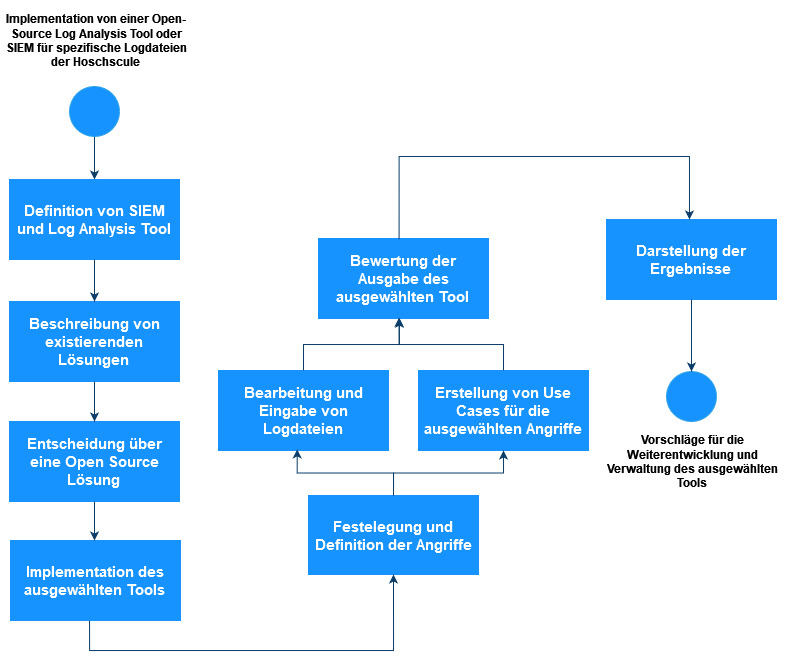
\includegraphics[width=1\textwidth]{assets/1_p1.jpg}
   \caption[Aufbau dieser wissenschaftlichen Recherche]
   {Aufbau dieser wissenschaftlichen Recherche \\Quelle: Eigene Darstellung }
   \label{fig:AblaufderArbeit}
   \centering
\end{figure}




  \section{Definition von SIEMs und Log-Analyse-Tools}

\gls{SIEM} ist das Ergebnis einer Kombination zwischen dem \glsfirst{SEM} und \glsfirst{SIM} \citep{Dorigo_SIEM}. Das Erste bezieht sich auf die Identifizierung, Bewertung, Beobachtung und Bericht von Sicherheitsvorfällen mithilfe von verschiedenen Log Dateien \citep{techopedia_SEM}. Das Zweite ist eine Software, die bei der automatischen Sammlung von Loginformationen aus vielen Quellen, wie Firewall und Servers unterstützt \citep{techopedia_SIM}. Da die meisten \gls{SIEM}-Lösungen kostenpflichtig sind, existieren auch viele \gls{opensource} Log-Analyse-Tools, die eine ähnliche Aufgabe erledigen, ohne die Kernelementen von \gls{SIEM} zu besitzen. 

Log-Analyse-Tools sind meistens Anwendungen die Logdateien empfangen, speichern, bearbeiten und nach spezifisichen eingegebenen Regeln bewerten. Diese Tools unterstützen Programmierer und Systemadministratoren bei der Überwachung des Zustands Systemen oder Software. Ein solches Tools kann Logdateien von verschiedenen \glsplural{Endpoint} und mit verschiedenen Formattierungen bekommen und editieren, so dass es schließlich ein Bericht oder Graphik erzeugt \citep{Korzeniowski_LATDef}. Die Nutzung dieser Tools schränkt sich nicht in dem Sicherheitsbereich ein, sondern kann für das gesamte Rechenzentren nützlich sein.


In dem Universum des \gls{SOC} mischen sich verschiedene Begriffe, die manchmal zur Verwirrung führen, weil sie ähnliche Bedeutung und Verantwortung haben. \glsfirst{IDS}, \glsfirst{IPS}, \glsfirst{SIEM} und Log-Analyse-Tools werden von \textit{nonnative users}  und sogar von Spezialisten oft verwechselt, da ihre Aufgaben mehr Zusammenhang als Unterschied haben. Um den Umfang dieser Arbeit wegen der zeitlichen Einschränkungen zu verringern, fassen wir kurz die Unterschiede zwischen denen zusammen und legen unsere Grenze auf den \glspl{SIEM} Lösungen und auf Log-Analyse-Tools fest. 

\newpage
\glsfirst{IDS} sind Software oder Hardware, die \glsplural{Cyberangriff} identifizieren und berichten. Sie haben eine passive Rolle, da sie die \glsplural{Cyberangriff} weder stoppen noch verhindern können. \glsfirst{IPS}allerdings haben eine aktive Haltung gegenüber \glsplural{Cyberangriff} - die können automatisch behandeln können, indem sie Blocking-Mechanismen einschalten, um den Angriff zu stoppen \citep{Wendzel_IS}. Wie das \gls{IDS}, kann das \gls{IPS} auch Logdateien generieren, die von einer \gls{SIEM}-Lösung gesammelt werden können. \glsplural{SIEM} können seinerseits die Logdateien von diesen und von anderen \glsplural{Endpoint} bekommen und diese nach vordefinierten Regeln bewerten, um dem \gls{SOC}-Team über Sicherheitsvorfälle zu informieren oder automatisch Maßnahmen zu ergreifen. Wie \glsplural{SIEM} bekommen Log-Analyse-Tools auch Logdateien, um Bericht oder Darstellung zu genieren. Ihre Nutzung ist aber nicht so spezifisch wie die von \glsplural{SIEM}. 

Die folgende Abbildung stellt didaktisch eine allgemeine Struktur von \gls{SIEM}-Lösungen dar:

\begin{figure}[H]
   \centering
   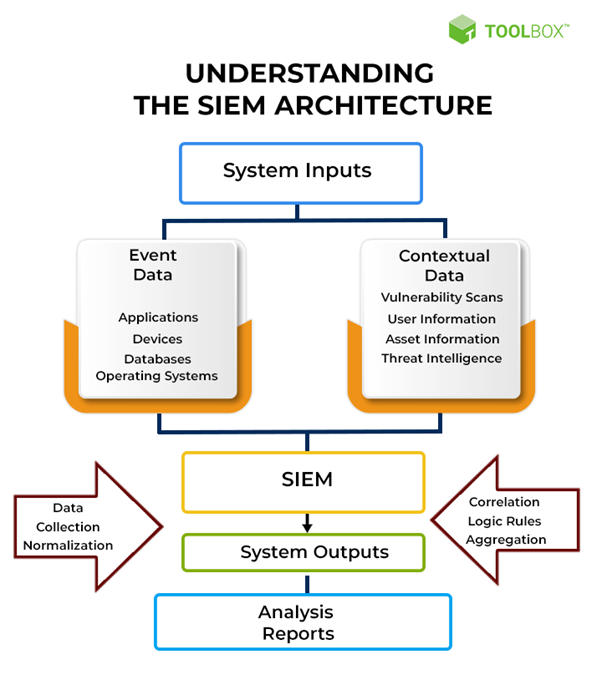
\includegraphics[width=0.55\textwidth]{assets/2_p1.png}
   \caption[Allgemeine Struktur von \gls{SIEM}]
   {Allgemeine Struktur von \gls{SIEM}\\Quelle: \citep{Mohanan_What} }
   \label{fig:SIEM_Allg_Struktur}
   \centering
\end{figure}

\newpage
Aus dem Bild können wir feststellen, dass \glsplural{SIEM} für die Zentralisierung von Sicherheitsdaten zuständig ist. Diese werden dann bearbeitet und in einem oder mehreren Berichten dargestellt, damit das \gls{SOC}-Team schnellere und effektive Entscheidungen treffen können. Der Informationsfluss einer \gls{SIEM}-Lösung können wieder in der folgenden Abbildung darstellen werden:

\begin{figure}[H]
   \centering
   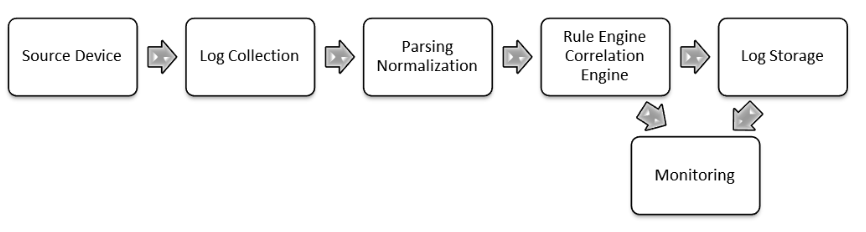
\includegraphics[width=0.8\textwidth]{assets/2_p2.png}
   \caption[Allgemeine Informationsfluss von \gls{SIEM}]
   {Allgemeine Informationsfluss von \gls{SIEM} \\Quelle: \citep{Granadillo_SIEM} }
   \label{fig:SIEM_Allg_Informationsfluss}
   \centering
\end{figure}

Die folgende Abbildung stellt eine allgemeine Architektur von Log-Analyse-Tools dar:

\begin{figure}[H]
   \centering
   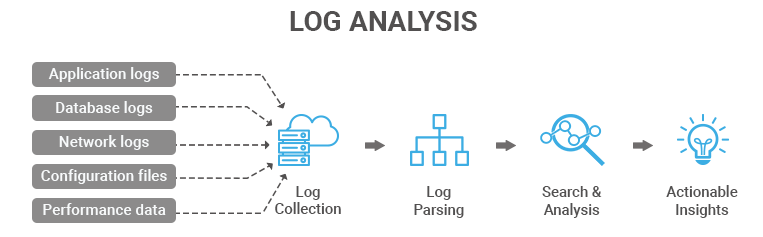
\includegraphics[width=0.8\textwidth]{assets/2.1_p2.png}
   \caption[Allgemeine Struktur von Log-Analyse-Tools]
   {Allgemeine Struktur von Log-Analyse-Tools\\Quelle: \citep{Tek-Tools_LGTArchitektur} }
   \centering
\end{figure}

Den Informationsfluss eines Log Analyst Tools bildet folgendes Bild ab:

\begin{figure}[H]
   \centering
   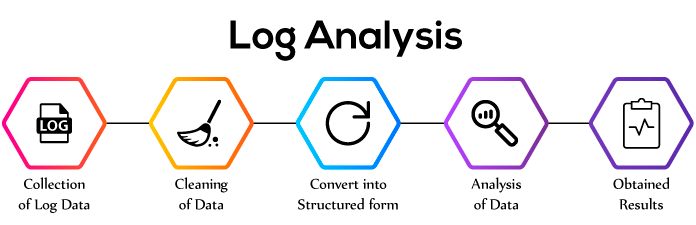
\includegraphics[width=0.55\textwidth]{assets/2.2_p2.png}
   \caption[Allgemeine Informationsfluss von Log-Analyse-Tools]
   {Allgemeine Informationsfluss von Log-Analyse-Tools\\Quelle: \citep{Neptune_LATInfoFluss} }
   \centering
\end{figure}

Aus bisheriger Beschreibung stellen wir fest, dass \gls{SIEM} viel mehr als eine Sammlung von Logdateien sind. Das Ziel dieser Software ist die automatische Analyse zu ermöglichen, indem Daten kombiniert und bewertet werden können. In vielen Bereichen, wie Finanzen (\glsfirst{PCDISS}), Gesundheitswesen (\glsfirst{HIPAA}), sind \glsplural{SIEM}s eine gesetzliche Verpflichtung \citep{Jog_SIEM}. In Deutschland verpflichtet das zweite Gesetz zur Erhöhung der Sicherheit informationstechnischer Systeme Organisationen mit kritischen Infrastrukturen die Anwendungen solcher Lösungen, um Störungen der \glsfirst{CIA} zu verhindern \citep{BSI_ITSG}. Log-Analyse-Tools sind seinerseits allgemeine Tools zu der Speicherung, Anpassung, Bewertung und Darstellung von Logdateien, ohne dass sie sich auf der Sicherheitsebenen fokussieren.


\subsection{Existierende SIEMs Lösungen und Log-Analyse-Tools}
% über Splunk schreiben, state of the art, nicht open source, aber andere müssen ähnliche funktionaliten haben
Die existierenden \glsplural{SIEM} und Log-Analyse-Tools können in zwei Kategorien getrennt werden: \textit{\gls{Proprietary}} und  \textit{\gls{opensource}}. In folgenden Abschnitten präsentieren wir die proprietäre \gls{SIEM} Splunk, um einen Maßstab für unsere Auswahl zu definieren, wenn es um Funktionalitäten geht. Wir analysieren folgende \glsplural{SIEM} und Log-Analyse-Tools: 

\begin{itemize}[noitemsep]
   \item Prelude %(nein)
   \item AlienVault \glsfirst{OSSIM} %(nein)
   \item FortiSIEM %(nein)
   \item ELK-Stack %(nein)
   \item Grafana %(ja)
\end{itemize}

%\textbf{\textcolor{red}{Wie konnte ich Grafana hier erwähnen? Grafane ist eher allgemein und nicht so zu Alert orientiert, habe ich hier gefunden: \href{https://www.metricfire.com/blog/grafana-vs-splunk/}{Splunk x Grafana} und hier \href{https://www.researchgate.net/publication/350730340_Implementation_of_Grafana_as_open_source_visualization_and_query_processing_platform_for_data_scientists_and_researchers}{What is Grafana}}  }

\newpage
\subsubsection{Splunk}
Splunk von dem Unternehmen Splunk Technology wurde 2003 in den USA veröffentlicht \citep{Splunk_splunk}. Er gehört weltweit zu der meistverwendeten \gls{SIEM}-Softwares und gilt als \textit{State of the art} für andere ähnliche Lösungen \citep{Kazarov_Splunk}. Zu ihren Kunden gehören große Konzerne wie Airbus, Coca-Cola, Intel und Deutsche Bahn. 

Splunk bietet laut seiner Webseite folgenden Funktionalitäten an \citep{Splunk_SPE}:

\begin{itemize}[noitemsep]
   \item Skalierbare Datenplattform 
   \item Risk-based Warnmeldung  
   \item Bedrohungserkennung mithilfe von \glsfirst{ML} 
   \item Automatische Aktualisierung von der Bedrohungs- und Schwachstelle-Database 
   \item Unkomplizierte Installation und Anwendung 
\end{itemize}

Die allgemeine Architektur und der Informationsfluss von Splunk unterscheiden sich nicht von den obigen dargestellten Struktur \ref{fig:SIEM_Allg_Struktur}, Seite \pageref{fig:SIEM_Allg_Struktur}, und Informationsfluss\ref{fig:SIEM_Allg_Informationsfluss}, Seite \pageref{fig:SIEM_Allg_Informationsfluss}. Da es sich hier um eine proprietäre Lösung handelt, lässt sich Splunk mit vielen anderen Funktionalitäten verwalten und erweitern. Das folgende Abbildung zeigt ein zusammenfassendes Diagramm über den Umfang des Informationsfluss von Splunk:

\begin{figure}[H]
   \centering
   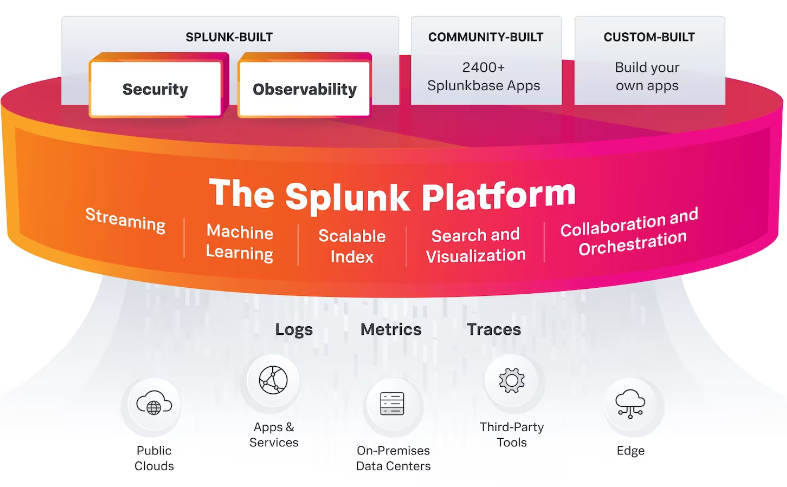
\includegraphics[width=0.7\textwidth]{assets/Splunk_informationsfluss.png}
   \caption[Allgemeine Informationsfluss von Splunk]
   {Allgemeine Informationsfluss von Splunk\\Quelle: \citep{Splunk_platform} }
   \centering
\end{figure}

In Splunk funktioniert die Bedrohungserkennung mithilfe von \glsplural{usecases}. Laut der Dokumentation existieren sie in folgenden Szenarien: Überwachung, Untersuchung und Erkennung. Die Software ist sowohl mit gls{mitre} Matrix als auch mit \glsfirst{CKC} für die Gestaltung ihrer \glsplural{usecases} integriert \citep{Splunk_usecases}. 

In einer spezifischen Arbeit wurden Angriffe auf einem System simuliert und schließlich mit Splunk analysiert, um Gefahren zu identifizieren und diese im Voraus zu sehen \citep{Su_SplunkDDOS}. In anderer Arbeit beschrieben die Autoren, wie eine Splunk-Instanz installiert und konfiguriert wurden, um spezifische \gls{bruteforce} zu erkennen \citep{Selvaganesh_SplunkBruteForce}.
 
\subsubsection{Prelude}
% suche nach Modulen, die man separat benutzen kann (Correlator)
Das im Jahr 2002 in Frankreich von Yoann Vandoorselaere freigegebene Tool Prelude zählt zu einer europäischen \gls{opensource} \gls{SIEM} Lösung. Laut dem Anbieter verfügt Prelude unter anderem folgende Funktionalitäten \citep{Prelude_SIEM}: 

\begin{itemize}[noitemsep]
   \item	Informationszentralisierung 
   \item	Datenaggregation und -Zusammenhang mit vordefinierten und von dem Nutzer angepassten Regeln 
   \item	Einbruchserkennungsmechanismen 
   \item	Datennormalisierung 
\end{itemize}

Die Anwendung besteht aus verschiedenen unabhängigen Modulen. Unter denen highlighten wir Warnmeldung, Archivierung, Analyse und Verwaltung. Das Erste gehört zu der zentralen Aufgabe dieser Lösung - es ist dafür zuständig, Daten zu empfangen, zu normalisieren, Zusammenhänge zu erschließen und Meldungen zu generieren. Das zweite Modul - Archivierung konzentriert sich auf die Speicherung und Verfügbarkeit der Daten. Zu dem Analyse-Modul gehören statistische Aufgabe und Darstellung in verschiedenen Formaten. Das letzte Modul dient dazu, die Anwendung zu steuern, Nutzer zu erstellen, dessen Rechte zu konfigurieren \citep{EC_Prelude}. 

Die folgende Abbildung zeigt die Integration verschiedener Module von Prelude und wie sie mit einander kommunizieren, um Analyse, Meldung und Speicherung zu generieren:

\begin{figure}[H]
   \centering
   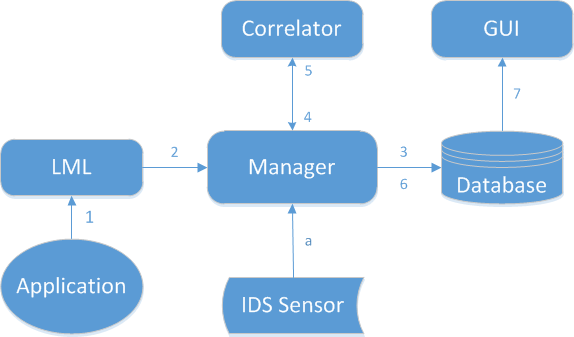
\includegraphics[width=0.5\textwidth]{assets/2_p3.png}
   \caption[Integration zwischen den Modulen von Prelude ]
   {Integration zwischen den Modulen von Prelude \\Quelle: \citep{Prelude_MU} }
   \centering
\end{figure}

Aus der Abbildung und der Dokumentation können wir folgenden Informationsfluss erkennen - die Daten werden von Endanwendung generiert und zum Loganalyzer (Prelude \glsfirst{LML}) geschickt, wo sie normalisiert und bewertet werden. Für solche Logs, wo es verdächtige Werte gibt, werden Warnmeldungen generiert. Diese Meldungen werden zum Manager Module weitergeleitet. Der Correlator oben sucht nach einem Zusammenhang zwischen anderen Daten. Das Ergebnis von Correlator wird wieder zum Manager geschickt und danach zu der Datenbank. Schließlich stehen die Berichte in dem User-Interface zur Verfügung \citep{Prelude_Doc}.

Die Architektur der Anwendung ermöglicht sowohl einen zentralisierten als auch einen dezentralisierten Aufbau. In der nächsten Abbildung sehen wir eine einfache Darstellung des Informationsfluss von Prelude:

\begin{figure}[H]
   \centering
   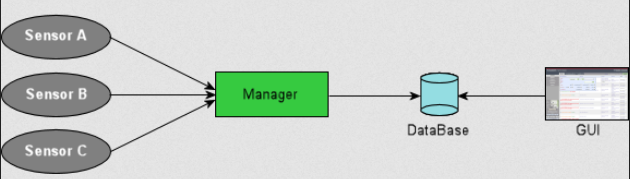
\includegraphics[width=0.7\textwidth]{assets/2_p4.png}
   \caption[Informationsfluss in Prelude]
   {Informationsflussin Prelude \\Quelle: \citep{Prelude_MU} }
   \centering
\end{figure}

In einer dezentralisierten Umgebung werden Daten von verschiedenen und getrennten Quellen generiert und bearbeitet. schließlich können die Nutzer auf diesen Daten unter einem \glsfirst{GUI} zugreifen.

\begin{figure}[H]
   \centering
   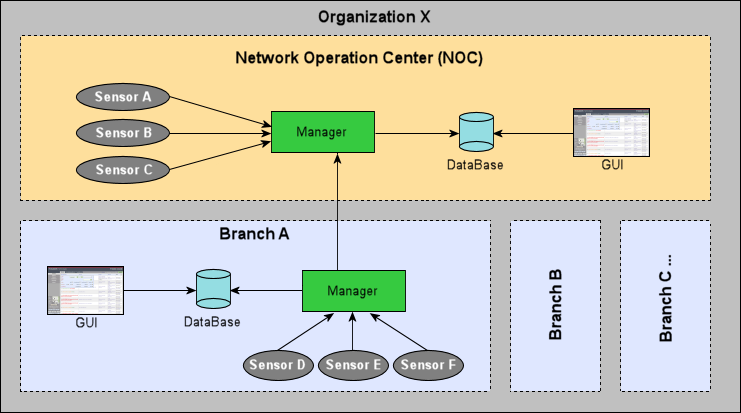
\includegraphics[width=0.8\textwidth]{assets/2_p5.png}
   \caption[Erweiterte Architektur von Prelude mit der Nutzung von dezentralisierten Datenquellen und Bearbeitung]
   {Erweiterte Architektur von Prelude mit der Nutzung von dezentralisierten Datenquellen und Bearbeitung\\Quelle: \citep{Prelude_MU} }
   \centering
\end{figure}

Die wissenschaftliche Literatur über Prelude ist sehr eingeschränkt. Wenige Publikationen fokussieren sich auf die Entwicklung, Implementation und unternehmerische Anwendung dieses Tools. Eine Studie von 2021 versuchte dieses und zwei andere Tools (AlienVault und Cyberoam iView) anhand technischer und nutzerfreundlicher Kriterien zu vergleichen. Unter diese Kriterien highlighten wir folgende\citep{Grammatikis_Prelude}: 

\begin{itemize}[noitemsep]
   \item \textbf{technische Kriterien}
   \begin{itemize}[noitemsep]
      \item \textit{Real-time performance}, 
      \item \textit{Range and flexibility of reporting}
      \item \textit{Alert correlation}
   \end{itemize}

   \item \textbf{nutzerfreundliche Kriterien}
   \begin{itemize}[noitemsep]
      \item \textit{Documentation comprehensiveness}
      \item \textit{Complexity of the installation process}
      \item \textit{Complexity of the system configuration}
   \end{itemize}
\end{itemize}

In den technischen Kriterien lag Prelude auf dem dritten Platz und in den benutzerfreundlichen Kriterien bekam Prelude den ersten. 

Auch in den nicht wissenschaftlichen Publikationen existiert eine begrenzte Anzahl von Texten über Preludes. Die existierenden Texte kommentieren ganz zusammenfassend die ausreichende Dokumentation und heben hervor, dass es eher eine in Europa konzentrierte Lösung ist.

\subsubsection{AlienVault OSSIM}
AlienVault OSSIM ist eine im Jahr 2007 entwickelte \gls{opensource} \gls{SIEM} Lösung. Im Jahr 2018 wurden sie von der Firma AT\&T Communication gekauft  \citep{CBN_AV}. In der Beschreibung des Anbieters steht, dass er sie auch dabei unterstützt, Daten zu sammeln, zu normalisieren und zu bewerten. Er behauptet auch, dass sein Tool in der Lage ist, Schwachstellen und Angriffe zu erkennen, das Verhältnis zu beobachten und Datenzusammenhang zu erschließen \citep{ATT_AVO}. 

AlienVault hat eine kostenpflichtige Version, die Alien Vault \glsfirst{USM} heißt. In der Webseite von AT\&T steht, dass es keine spezifische Dokumentation für die \gls{opensource} Version, AlienVault OSSIM, gibt, da viele Funktionalitäten von der anderen Version stammen \citep{ATT_AVO}. 

\newpage
Die folgende Abbildung zeigt das von dem Anbieter freigelegte Architekturdiagramm von der \gls{USM} Version:

\begin{figure}[H]
   \centering
   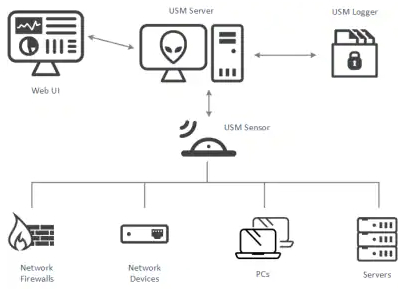
\includegraphics[width=0.6\textwidth]{assets/2_p6.png}
   \caption[Architekturdiagramm von AlienVault \gls{USM}]
   {Architekturdiagramm von AlienVault \gls{USM} \\Quelle: \citep{ATT_AVO} }
   \centering
\end{figure}

Laut der Website Comparitech steht AlienVault in der 13ten Platz von den besten bewerteten \gls{SIEM}-Lösungen. Die Seite beschreibt auch, dass zu dem Tool einen \gls{IDS}, ein Verhaltensüberwachungssystem und einen Schwachstellen-Scanner integriert sind. Die Anwendung ist auch mit der Plattform \gls{OTX} verbunden - diese ermöglicht eine Teilung von Informationen über die Schwachstelle. Comparitech highlighted, dass die Anwendung wegen ihrer niedrigen Kosten besser für kleine oder mittelständige Unternehmen geeignet ist \citep{comparitech_SIEM}. 

Die Anwendung soll konsistenten Daten Zusammenhang anbieten und soll das Auftauchen von \gls{falsch positiv} vermeiden. AlienVault kommt auch mit vordefinierten Use-Cases, die dabei unterstützen, gewöhnlichen Angriffsszenario zu erkennen. Die Installation, die Einstellung und die Integration mit anderen Tools ist auch benutzerfreundlich \citep{Gomes_AV}. Aus einer anderen wissenschaftlichen Quelle fanden wir heraus, dass für viele Quellen eine manuelle Normalisierung der Logdatein notwendig ist \citep{Nabil_AV}. Die Anwendung hat aber einen zuverlässigen Berichtsmechanismus. 

Während unserer Recherche gab es wenig wissenschaftliche Literatur, die sich um AlienVault OSSIM kümmert. Die meisten Publikationen waren aus kommerziellen Quellen und diese konzentrierten sich auf eine kostenpflichtige \gls{SIEM}-Lösung von AT\&T..

\subsubsection{FortiSIEM}
FortiSIEM ist eine US-amerikanische \gls{SIEM}-Lösung von der Firma Fortinet. Fortinet kaufte im Jahr 2016 das Unternehmen AccelOps und dessen \gls{SIEM}-Lösung und benannte es zum FortSIEM \citep{Fortinet_Press}. 

Laut dem Anbieter hat FortiSIEM eine robuste Integration mit anderen Tools und lässt sich leicht und einwandfrei skalieren. Andere Versionen des Tools sind mit \glsfirst{ML} integriert, sodass die Anwendung auch Verhältnisanalyse durchführen kann \citep{Fortinet_Solutions}. Das Tool bietet auch eine umfangreiche und ausführliche Dokumentation an. Die nächste Abbildung zeigt die skalierbare Architektur des Tools:

\begin{figure}[H]
   \centering
   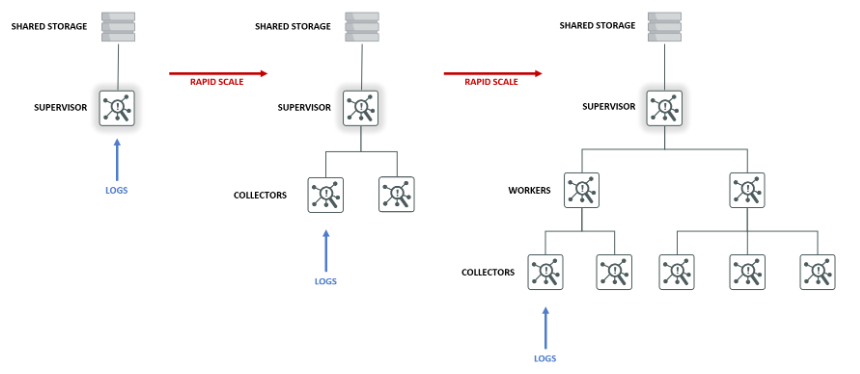
\includegraphics[width=1\textwidth]{assets/2_p7.png}
   \caption[Skalierbare Architektur von FortiSIEM]
   {Skalierbare Architektur von FortiSIEM \\Quelle: \citep{Fortinet_Arch} }
   \centering
\end{figure}

\newpage
Auch zu dieser \gls{SIEM}-Lösung ist die wissenschaftliche Produktion eingeschränkt. Eine von der gefundenen Publikation betont, dass FortiSIEM eine schnelle Erkennung von Angriffen anbietet und über  \glsfirst{NOC} Funktionalitäten verfügt \citep{Ramires_fortisiem}. Wie andere \glspl{SIEM} Lösungen, hat FortiSIEM folgende Funktionalitäten:

\begin{itemize}[noitemsep]
   \item Datensammlung und Normalisierung
   \item Daten Zusammenhang
   \item Generierung von Berichten
   \item Warnmeldungen
   \item Datenauswertung
\end{itemize}

\subsubsection{ELK-Stack}
ELK Stack stammt aus der Verbindung von drei Tools: Elasticsearch, Logstash und Kibana. Das Erste ist eine Such-und Analyse-Maschine. Das Zweite ist eine serverseitige Anwendung zur Datenverarbeitung und -Weiterleitung. Schließlich Kibana \label{kibana} ist dafür zuständig, visuelle Darstellung in Grafik-Format auszugeben (packt, 2019). Von diesen drei Tools Logstasch ist der einzige \gls{opensource} \citep{elastic_OSI}. Obwohl die anderen zwei 
kostenlos verwendet werden können, gehören sie nicht zu der \gls{opensource} Kategorie \citep{OpenSource_Def}. Dieses Tool besitzt viele Eigenschaften einer \gls{SIEM}-Lösung und wird von vielen SOC verwendet, ist aber, für viele Experten, kein \gls{SIEM} für sich, da es über keine Warnmeldungssystem, Daten Zusammenhang und Vorfälleverwaltung verfügt \citep{Miller_ELK}. Diese und anderen Funktionalitäten lassen sich aber durch \glsplural{plugin} integrieren. 

\newpage
Das folgende Diagramm stellt die Architektur von ELK Stack mit ihren integrierten Elementen dar:

\begin{figure}[H]
   \centering
   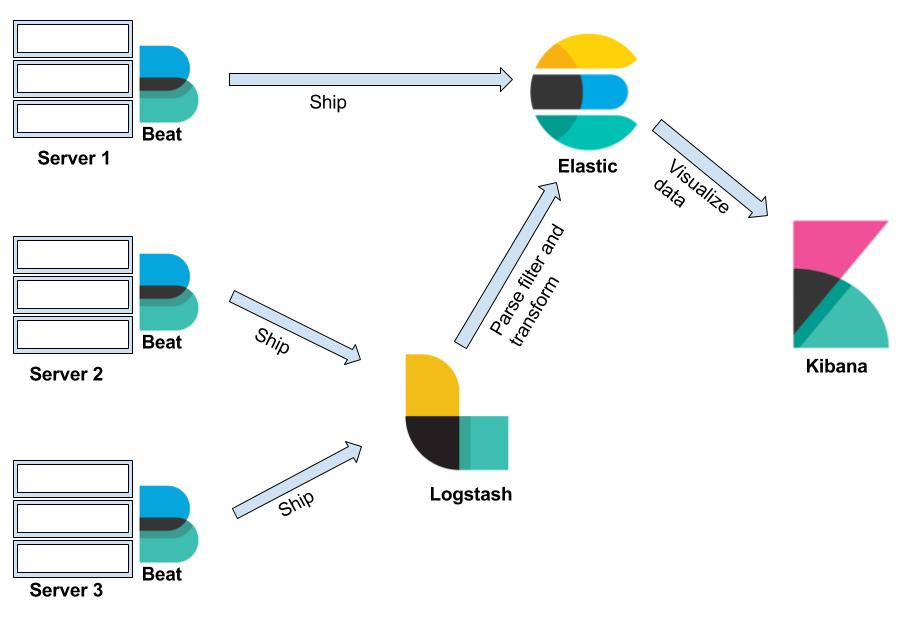
\includegraphics[width=0.8\textwidth]{assets/2_p8.png}
   \caption[Integration zwischen Elasticsearch, Logstash und Kibana]
   {Integration zwischen Elasticsearch, Logstash und Kibana\\Quelle: \citep{packt_elkstack} }
   \centering
\end{figure}

Die Beats auf dem Bild sind an der \glsplural{Endpoint} installiert und leiten Daten entweder zu Elasticsearch oder zu Logstash weiter, wo sie schließlich bearbeitet werden \citep{Jain_LMELK}. 

Ein Teil der wissenschaftlichen Literatur zeigt die Log Analyse-Funktionalitäten von ELK Stack und die Unterstützung bei Normalisierung und Indexierung von Daten für eine lesbare Ausgabe \citep{Advani_elkstakc}. Die starke Skalierbarkeit wurde auch bei einer Studie erwähnt, wo ELK Stack für Wi-Fi Logging eingesetzt wurde \citep{Wang_elkwifi}. 

Die offizielle Dokumentation von ELK Stack betont, dass die Anwendung folgende Funktionalitäten besitzt \citep{elastic_docs}: 

\begin{itemize}[noitemsep]
   \item Datensuche, -Normalisierung, -Analyse und 
   \item Speicherung
   \item visuelle Ausgabe
\end{itemize}

Folgendes Diagramm aus der offiziellen Dokumentation zeigt die Aufteilung der Funktionalitäten pro Element von ELK Stack:

\begin{figure}[H]
   \centering
   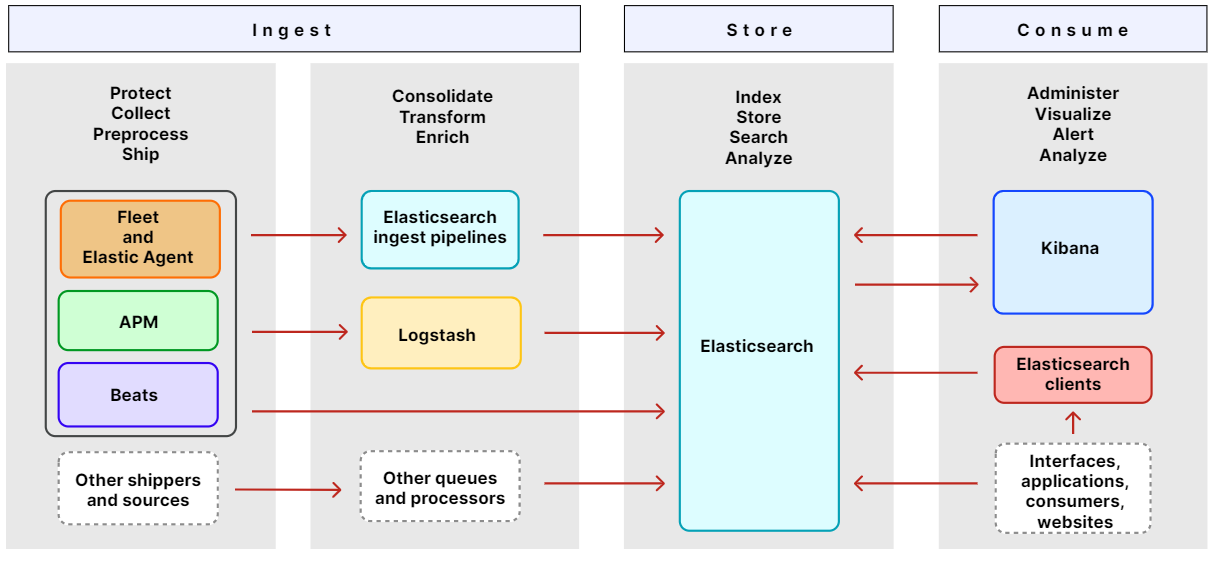
\includegraphics[width=0.8\textwidth]{assets/2_p9.png}
   \caption[Aufteilung der Funktionalitäten zwischen den Komponenten]
   {Aufteilung der Funktionalitäten zwischen den Komponenten\\Quelle: \citep{elastic_docs}}
   \centering
\end{figure}

Die wissenschaftliche Publikation über ELK-Stack ist vielfältiger als bei anderen recherchierten Tools. Es ist aber wichtig, zu betonen, dass die Mehrheit von denen sich eher mit dem Logging als mit den \gls{SIEM}-Eigenschaften der Anwendung beschäftigt.

\subsubsection{Grafana}
Von allen recherchierten Lösungen ist Grafana die Einzige, die nicht als \gls{SIEM} dargestellt ist. Grafana wird aber als Plattform für Visualisierung von Data beschrieben. Mit dem Tool ist es möglich eine Graphik zu erstellen und Meldungen zu definieren. Das Ziel der Anwendung ist, Information in einer einfachen und verständlichen Art und Weise zur Verfügung zu stehen \citep{redhat_grafana}.  

Im Jahr 2014 wurde Grafana von der Firma Grafana Labs veröffentlicht. Das Tool basiert auf Kibana3,\ref{kibana}. Ursprünglich sollte Grafana ein einfacheres Editingstool für Graphik sein und ermöglichen, Datenanfragen unkomplizierter zu machen. Die neuste Version, 9.4.3. wurde im März 2023 veröffentlicht und bietet viele Funktionalitäten an. Es ist auch möglich das Tool mithilfe von  \glsplural{plugin} zu erweitern \citep{Oedegaard_historyGrafana}.. 

In der Webseite betont der Anbieter, dass Grafana die Zentralisierung und Zugang von Daten vereinfachen. Alle Art von Daten lassen sich analysieren und darstellen, von der Leistung von Anwendungen bis Verkaufsdaten und Krankheitsfällen. Die Anwendung soll auch den Zusammenhang von Daten ermöglichen, um wichtige Informationen herauszunehmen \citep{Grafana_Grafana}.

Grafana ist auch mit dem Logging Tool Loki und Promptail integriert. Promtail ist für Sammlungen der Logdateien und Weiterleitung an Loki zuständig. Promptail wird an jeden \gls{Endpoint} installiert. In Loki werden diese Logdateien ohne Index für den schnellen Zugriff gespeichert. Diese Daten können dann in Grafana mithilfe der \gls{abfragesprache} LogQL aufgerufen werden. Schließlich können Warnmeldung mit spezfisichen Regel generiert werden, die in Loki eingeführt werden \citep{Grafana_loki}. Auf dem Folgenden Bild wird die Struktur von Grafana Loki  dargestellt:

\begin{figure}[H]
   \centering
   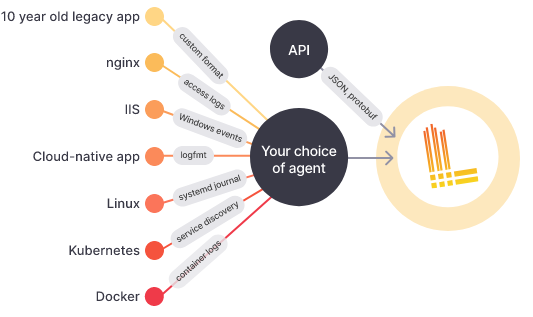
\includegraphics[width=0.8\textwidth]{assets/2_p10.png}
   \caption[Integration von Log-Quellen mit Grafana Loki und Promptail]
   {Integration von verschiedenen Log-Quellen mit Grafana Loki und Promptail \\Quelle: \citep{Grafana_Logs}}
   \centering
\end{figure}

Das Tool hat auch eine umfangreiche Dokumentation, die ausführlich erklärt, wie sie sich installieren, bedienen und mit anderen Tools integrieren lässt. 

%\newpage
%Obwohl Grafana nicht spezifisch für den Sicherheitsbereich konzipiert wurde, kann das Tool so eingerichtet werden, dass spezifische Logdateien gesammelt, bearbeitet und analysiert werden. Die Warnmeldung lässt sich mit Regeln oder Filter definieren. In einer Recherche von 2022 wurde Grafana dafür benutzt, Daten aus Netzwerkverkehr graphisch darzustellen \citep{Manases_grafananetwork}. 

Die wissenschaftlichen Literatur über Grafana konzentriert sich eher auf die Anwendung des Tools für die graphische Darstellung von Daten als für ihre Nutzung in dem Sicherheitsbereich. Einw Recherche, z.B., wollte das Ergebnis von der Überwachung von Cloud-Based Systemen, von Netzwerkaktivitäten und von Netzwerkverkehr mithilfe von Grafana darstellen \citep{Manases_grafananetwork}. In dieser Hinsicht gibt es wenige wissenschaftliche Arbeit, wo die Implementation und Integration von Grafana mit anderen Tools für den Sicerheitsbereich die Hauptfigur ist.

\subsection{Auswahlkriterien}
Eine umfangreiche \gls{SIEM} Software die viele automatische Lösung für die Erkennung und Bekämpfung von Cyberangriffe würde perfekt für jede Situation passen. Da solche Lösungen meistens (oder alle) \gls{Proprietary} sind und nur für teure Preise angeboten werden, entschieden wir uns für die Anpassung an einem \gls{opensource}Tool, das zu unserem Kontext und Einschränkungen gehört. 

Demnächst beschäftigen wir uns mit Grafana. Wir beschreiben, wie wir das Tool installieren, konfigurieren und mit verschiedenen Logdateien eingeben. Nachdem die Grundfunktionalitäten eingerichtet sind und einwandfrei funktionieren, generieren wir anhand der \gls{mitre} Matrix \glsplural{usecases} für die zukünftigen ausgewählten Angriffe. Unser Ziel ist Grafana so einzustellen, dass es in der Lage ist, die Muster dieser Angriffe zu erkennen und darüber zu berichten.

  \section{Implementierung}
In diesem Kapitel geht es um die Implementierung und den Aufbau von Grafana, um \gls{Cyberangriff} mithilfe der \gls{mitre} Matrix zu erkennen. Das Labor wird mit einem \gls{container} und \glsfirst{vm} aufgebaut, wie im Diagramm in der Abbildung \ref{fig:Arbeitslabor} dargestellt.

\begin{figure}[H]
   \centering
   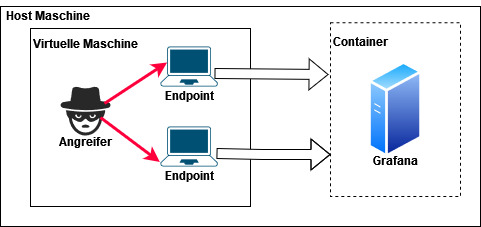
\includegraphics[width=1\textwidth]{assets/Arbeitslabor.jpg}
   \caption[Aufbau unseres Arbeitslabors]
   {Aufbau unseres Arbeitslabors \\Quelle: Eigene Quelle}
   \label{fig:Arbeitslabor}
   \centering
\end{figure}

Unser Aufbau verfolg folgende Ziele: die Aufnahme und Anpassung von Logdateien für Grafana, die Mustererkennung für ausgewählte \glsplural{Cyberangriff} und schließlich die Erstellung von Warnmeldungen für die Endnutzer, damit sie geeignete Sicherheitsmaßnahmen ergreifen können.

\newpage
Der gezielte Ablauf unserer Arbeit ist in der Abbildung \ref{fig:Ablauf_grafana2} dargestellt:

\begin{figure}[H]
   \centering
   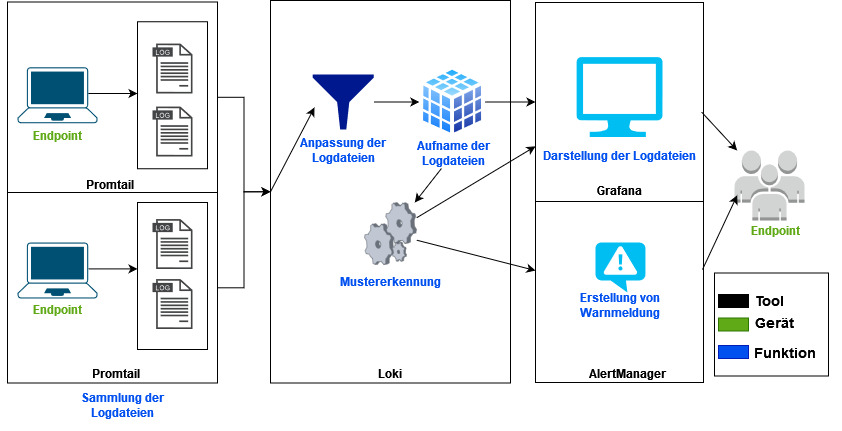
\includegraphics[width=1\textwidth]{assets/Ablauf_grafana2.jpg}
   \caption[Erwarteter Ablauf der Sammlung der Logdateien bis zur Warnmeldung]
   {Erwarteter Ablauf der Sammlung der Logdateien bis zur Warnmeldung \\ Quelle: Eigene Quelle und \citep{Grafana_loki}}
   \label{fig:Ablauf_grafana2}
   \centering
\end{figure}

\subsection{Angriffserkennung anhand der Mitre ATT\&CK Matrix}
Es gibt verschiedene Methoden und Frameworks, die von \gls{SOC}-Teams verwendet wird, um \glsplural{Cyberangriff} zu vermeiden, zu erkennen und zu unterbrechen.  Da sich die Richtlinien und Schwerpunkte dieser Frameworks und Methoden unterscheiden können und somit unterschiedliche Anforderungen an den Aufbau unserer Struktur stellen könnten, entschieden wir uns für die \gls{mitre} Matrix, insbesondere da dieses Framework auch in Splunk integriert ist. 

Die \gls{mitre} Matrix hat folgenden Zwecke \citep{Mitre_Started}:

{\setstretch{1.5}
\begin{itemize}[noitemsep]
   \item Erkennung und Analyse von Angriffstechnik
   \item	strukturierte Datensammlung über Bedrohungen
   \item	Emulieren von \glsplural{Cyberangriff} für die Anwendung an Angriffsübungen
   \item	Systemhärtung und Verbesserung der Verteidigungsmaßnahmen
\end{itemize}
}

Die Matrix ermöglichen Unternehmen und \gls{SOC}-Teams umfassende Möglichkeiten, um ihre Ressourcen zu schützen und ihr Fachwissen im Bereich der \gls{Cybersicherheit} zu erweitern \citep{Hazel_howtousemitre}. In dieser Arbeit konzentrieren wir uns auf die Entwicklung und Implementierung einer Methode zur automatischen Erkennung und Analyse von Angriffstechniken in Grafana.

Die \gls{mitre} Matrix ist auf \glsfirst{ttp} basiert. Angriffe, Gegenmaßnahmen und Erkennung werden nach \gls{ttp} definiert. Die Matrix besteht aus 14 Taktiken, zu denen jeweils Techniken gehören, die wiederum in Sub-Techniken unterteilt sind. Jede Sub-Technik wird mit Beispielen, Härtungsmaßnahmen und Erkennungsregeln beschrieben. Die nächste Abbildung, \ref{fig:ttp}, zeigt, wie die \gls{ttp} aufgebaut werden:

\begin{figure}[H]
   \centering
   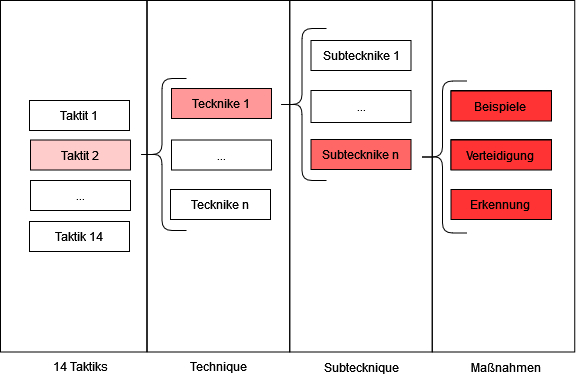
\includegraphics[width=0.8\textwidth]{assets/Mitre_structure.drawio.png}
   \caption[Struktur der \gls{mitre} Matrix]
   {Struktur der \gls{mitre} Matrix \\Quelle: Eigene Quelle und \citep{Mitre_Started}}
   \label{fig:ttp}
   \centering
\end{figure}

% {\setstretch{1}
% Die 14 Taktiks sind folgende:
% \begin{itemize}[noitemsep]
%    \item Informationssammlung für zukünftige Angriffe 
%    \item	Entwicklung von Ressource von Angreifer
%    \item Erster Zugang zum Opfersysteme 
%    \item Ausführung von bösartigen Coden
%    \item Beharrlichkeit von System
%    \item	Privilegienausweitung
%    \item Vermeidung von Verteidigungssysteme
%    \item \textbf{Zugang zu Anmeldedaten}
%    \item Umgebungserkennung
%    \item Seitliche Bewegung zu anderem Systemen innerhalb des Angriffsziels
%    \item interne Informationssammlung
%    \item Steuerung und Kontrolle (C2 - Command and Control im Original)
%    \item Datenextrahierung 
%    \item	Auswirkung auf die Integrität
% \end{itemize}
% }

\newpage
\subsection{Auswahl des Angriffes}
In dieser Arbeit beschäftigen wir uns mit der Taktik \quotes{Zugang zu Anmeldedaten} und deren Technik \gls{bruteforce}. Diese Technik ist in vier Untertechniken aufteilt:

In dieser Arbeit beschäftigen wir uns mit der Taktik \quotes{Zugang zu Anmeldedaten} und ihrer Technik \quotes{\gls{bruteforce}}. Diese Technik ist in vier Untertechniken unterteilt:

{\setstretch{1}
\begin{itemize}[noitemsep]
   \item \gls{bruteforce}
   \item	Entschlüsselung von \glsplural{hash}
   \item \textit{\gls{stuffing}}
   \item \textit{\gls{spraying}}
\end{itemize}
}

Da unser Ziel hier ist, Grafana zu verwenden, um Angriffe zu erkennen, haben wir uns für einen einfachen und reproduzierbaren Angriff entschieden, der wenige Ressourcen erfordert. In diesem Fall kann ein \gls{bruteforce} mit zwei \glsplural{vm} problemlos durchgeführt werden. Für diesen Angriff verwenden wir die Sub-Technik "Erraten von Anmeldedaten und \textit{\gls{stuffing}}, da sie ähnliche Erkennungsmethoden aufweisen. Da unser Fokus bei dieser wissenschaftlichen Arbeit auf der Angriffserkennung schließen andere Maßnahmen  wir hierbei aus.

Die nächste Abbildung, \ref{fig:Unser_ttp}, zeigt den Umfang unseres Implementationsversuchs mithifel von \gls{mitre}:
\begin{figure}[H]
   \centering
   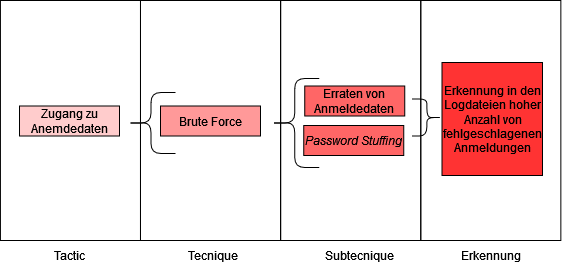
\includegraphics[width=0.7\textwidth]{assets/T1110.drawio.png}
   \caption[\glsfirst{ttp} für unseren Angriff]
   {\glsfirst{ttp} für unseren Angriff \\Quelle: Eigene Quelle und \citep{Mitre_t1110}}
   \label{fig:Unser_ttp}
   \centering
\end{figure}

\newpage
\subsection{Installation und Generierung von Logdateien}
In diesem Abschnitt konzentrieren wir uns auf die folgenden Punkte:

\begin{enumerate}[noitemsep]
   \item Einrichtung von \glsplural{vm} für das Opfersystem und den Angreifer
   \item Simulation des Angriffe zur Erzeugung von Logdateien
   \item Installation und Konfiguration von Grafana Loki und Promtail mit \gls{container}
   \item Weiterleitung der Logdateien an Grafana
\end{enumerate}

Die Installation und Verwendung können entweder über eine \glsfirst{GUI} des Betriebssystems oder über die Kommandozeile durchgeführt werden. In dieser Arbeit verwenden wir die Kommandozeile.

\subsubsection{Einrichtung der \glsplural{vm} für Opfersystem und Angreifen}
Die beiden \glsplural{vm} sind eine \quotes{\gls{kali} \glsfirst{vm}} und \quotes{\gls{ubuntu} Server 22.04.2} mit standardmäßigen Einstellungen. Beide Maschinen wurden entsprechend ihrer jeweiligen Dokumentation installiert \citep{kali_vm} und \citep{Ubuntu_server}.

Für das Opfersystem haben wir uns für die Passwörter \quotes{qwertz} und \quotes{password} entschieden. Laut einer Umfrage gehören diese Passwörter zu den zehn am häufigsten verwendeten Passwörtern in Deutschland \citep{silicon_passwort}. Für die Durchführung des \gls{spraying} haben wir folgende Benutzername-Passwort Kombinationen erstellt:

{\setstretch{1.0}
\begin{lstlisting}[frame=single]
            Opfersystem 1          Opfersystem 2  
            admin:123456           bob:hallo
            user1:passwort         master:alice
            user2:abc123           hans:daniel
            user3:qwertyuiop       bruno:super123
\end{lstlisting}
}

\newpage
\subsubsection{Generierung von Logdateien mit der Angrifsssimulation}
Für den Angriff verwenden wir folgende Tools:

{\setstretch{1.0}
\begin{itemize}[noitemsep]
   \item	\glsfirst{ssh}
   \item \gls{hydra}
\end{itemize}
}

In diesem Szenario sendet \gls{hydra} gleichzeitig mehrere Authentifizierungsversuche an das Opfersystem, um eine \gls{ssh}-Verbindung herzustellen. Das Tool verwendet ein sogenanntes Wörterbuch mit verschiedenen Einträgen, die als Passwörter dienen. Für unseren Test benutzen wir die bekannte \gls{rockyou}-Wörterbuch.

Die Abbildung \ref{fig:stuffing} zeigt, wie das \gls{stuffing} abläuft:
\begin{figure}[H]
   \centering
   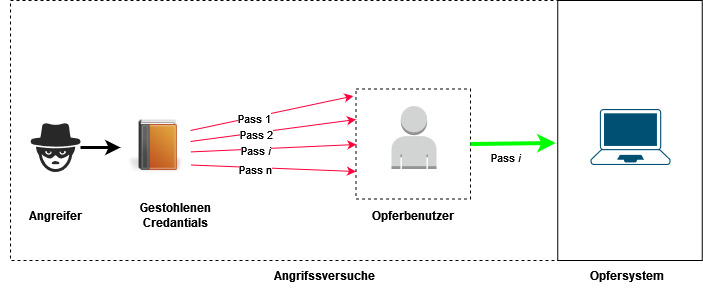
\includegraphics[width=1\textwidth]{assets/Stuffing.jpg}
   \caption[Darstellung von \textit{\gls{stuffing}}]
   {Darstellung von \textit{\gls{stuffing}}\\Quelle: Eigene Quelle und \citep{Nguyen_stuffing}}
   \label{fig:stuffing}
   \centering
\end{figure}

In diesem Angriff versucht der Angreifer sich mit einem Konto anzumelden, indem er mit vielen Passwörter aus dem Wörterbuch probiert, bis eins richtige gefunden ist. Es können mehrere Anmeldungsversuche geschickt werden, bis eine von denen funktioniert.

\newpage
\gls{stuffing} wurde mit folgendem Kommando durchgeführt \citep{kali_hydra}:
%Verbatim
{\setstretch{1.0}
\begin{Verbatim}[frame=single]
hydra -l [Benutzername] -P rockyou.txt [Opfersystem] ssh -V -t 4

# Erklärung
-l: Spezifikation des Benutzernamens, den wir angreifen
-P: Auswahl der Datei mit bekannten Passwörtern
ssh: Auswahl der Anwendung, die wir angreifen
-V: Ausführliche Ausgabe über Versuche, Fehler und Erfolg
-t 4: Anzahl von gleichzeitigen Verbindungen
\end{Verbatim}
}

Die Abbildunge \ref{fig:Ausgabe_Stuffing_Opfer1} und \ref{fig:Ausgabe_Stuffing_Opfer2} zeigen ein Teil der Ausgabe von \gls{hydra} während der Ausführung von \gls{stuffing} gegen das Opfersystem1 und Opfersystem2:
\begin{figure}[H]
   \centering
   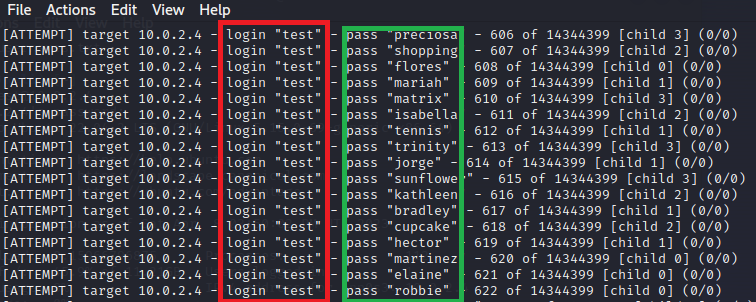
\includegraphics[width=0.9\textwidth]{assets/stuffing_kali.png}
   \caption[Ausgabe von \textit{\gls{stuffing}} gegen Opfersystem1]
   {Ausgabe von \textit{\gls{stuffing}} gegen Opfersystem1}
   \label{fig:Ausgabe_Stuffing_Opfer1}
   \centering
\end{figure}

\begin{figure}[H]
   \centering
   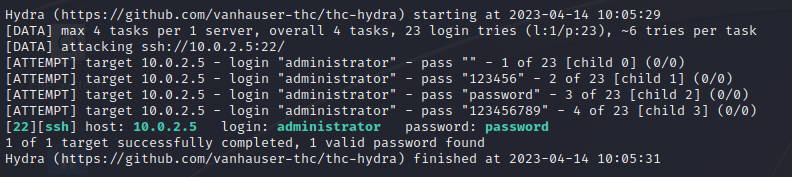
\includegraphics[width=1\textwidth]{assets/stuffing_kali2.png}
   \caption[Ausgabe von \textit{\gls{stuffing}} gegen Opfersystem2]
   {Ausgabe von \textit{\gls{stuffing}} gegen Opfersystem2}
   \label{fig:Ausgabe_Stuffing_Opfer2}
   \centering
\end{figure}

Auf den Abbildungen \ref{fig:Ausgabe_Stuffing_Opfer1} und \ref{fig:Ausgabe_Stuffing_Opfer2} sehen wir in rot markiert, dass der Angriff den Benutzernamen \quotes{test} im Opfersystem1 und \quotes{Administrator} Opfersystem2 zielt. In grün werden die verschiedenen Passwörter aus \gls{rockyou}-Wörterbuch verwendet. Auf der Abbildung \ref{fig:Ausgabe_Stuffing_Opfer2} wird das gefundene Passwört grün geschrieben. 

Unser nächster Angriff, \gls{spraying}, ist in der Abbildung \ref{fig:spraying} dargestellt:
\begin{figure}[H]
   \centering
   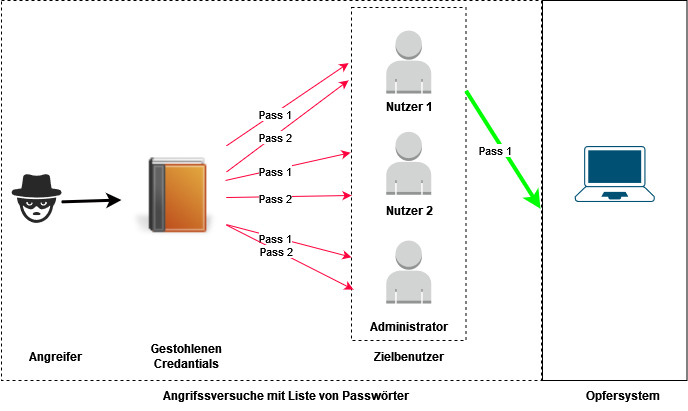
\includegraphics[width=0.9\textwidth]{assets/Spraying.jpg}
   \caption[Darstellung von \textit{\gls{spraying}}]
   {Darstellung von \textit{\gls{spraying}}\\Quelle: Eigene Quelle und \citep{Swathi_spraxy}}
   \label{fig:spraying}
   \centering
\end{figure}

Aus der Abbildung \ref{fig:spraying} sehen wir, dass bei \gls{spraying} weniger Passwörter im Vergleich zum \gls{stuffing} verwendet werden. In diesem Fall werden gegen mögliche viele existierenden Benutzername versucht. Hier will der Angreifer  Kontosperrungen vermeiden und gegenüber Sicherheitsmaßnamen Unauffälig bleiben. 

Für diesen Angriff benutzen wir folgendes Kommando:
{\setstretch{1.0}
\begin{Verbatim}[frame=single]
hydra -L username2.txt -P passwoerter.txt [Opfersystem2] ssh -V -t 4
-L: Auswahl der Datei mit gefunden Benutzernamen
\end{Verbatim}
}

In diesem Fall gehen wir davon aus, dass der Angreifer einige oder alle Benutzernamen bereits kennt. Da bei diesem Angriff weniger Anmeldeversuche pro Nutzer durchgeführt werden, verwenden wir eine selbst erstellte Datei mit weniger Passwörtern als die \gls{rockyou}-Datei. Unsere Datei enthält die am häufigsten verwendeten Passwörter in Deutschland \citep{silicon_passwort}.

Die Abbildungen \ref{fig:spraying_opfer1} und \ref{fig:spraying_opfer2} zeigen die Ausgabe von \gls{spraying}:
\begin{figure}[H]
   \centering
   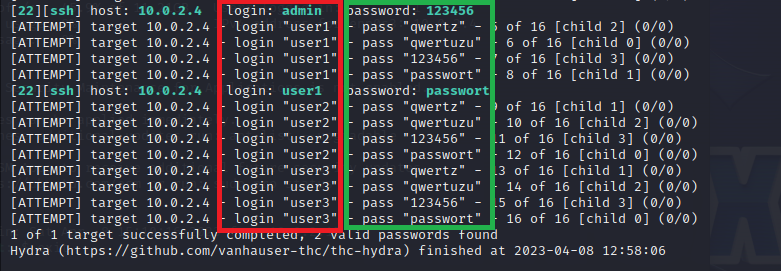
\includegraphics[width=1\textwidth]{assets/Spraying_Kali.png}
   \caption[Ausgabe von \textit{\gls{spraying}} in Kali Linux gegen Opfersystem1]
   {Ausgabe von \textit{\gls{spraying}} in Kali Linux gegen Opfersystem1}
   \label{fig:spraying_opfer1}
   \centering
\end{figure}

\begin{figure}[H]
   \centering
   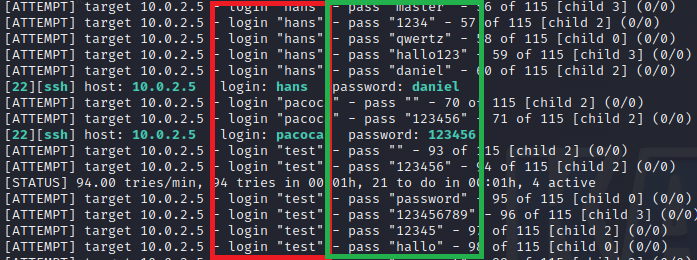
\includegraphics[width=1\textwidth]{assets/Spraying_Kali2.png}
   \caption[Ausgabe von \textit{\gls{spraying}} in Kali Linux gegen Opfersystem2]
   {Ausgabe von \textit{\gls{spraying}} in Kali Linux gegen Opfersystem2}
   \label{fig:spraying_opfer2}
   \centering
\end{figure}

Die Abbildungen \ref{fig:spraying_opfer1} und \ref{fig:spraying_opfer2} zeigen die verschiedenen Benutzername (rot markiert) aber wenige Passwörter pro Nutzer (grün markiert). Auf beiden Abbildungen werden die gefundenen Passwört grün geschrieben.

\newpage
\subsubsection{Installation und Einrichtung von Grafana Loki und Promtail}
Die offizielle Dokumentation von Grafana war nicht immer eindeutig in Bezug auf die Ausführung, daher haben wir auch auf externe Quellen zurückgegriffen, um die Einstellungen an unsere Umgebung anzupassen \citep{Polinowski_PGL}. Unten befinden sich die von Grafana zur Verfügung gestellten Konfigurationsdateien und Installationsverfahren \citep{GrafanaLoki_run}:

{\setstretch{1.0}
\begin{lstlisting}[frame=single]
wget https://raw.githubusercontent.com/grafana/loki/v2.8.0/cmd/
loki/loki-local-config.yaml -O loki-config.yaml
(die Datei wurde angepasst)

wget https://raw.githubusercontent.com/grafana/loki/v2.8.0/
clients/cmd/promtail/promtail-docker-config.yaml
-O promtail-config.yaml (die Datei wurde angepasst)

docker-compose -f docker-compose.yaml up 
\end{lstlisting}
}

Im Anhang \ref{appendix:orgGrafana} befinden sich die heruntergeladenen originalen Konfigurationsdatei. Ihre an unserer Umgebung angepassten Version steht im Anhang \ref{appendix:AngepasstGrafana} zur Verfügung.

Die obigen Kommandos haben folgende Bedeutungen:
\begin{enumerate}[noitemsep]
   \item Herunterladen der Konfigurationsdatei von Loki
   \item Herunterladen der Konfigurationsdatei von Promptail
   \item Ausführung von dem \glsplural{container}, indem beide Konfigurationsdateien in eine eingepackt und angepasst wurden und schließlich von der \gls{container}-Anwendung gelesen werden
\end{enumerate}

%Für spezifische Versionen oder weitere Einstellungen bietet die Dokumentation umfangreiche Möglichkeiten an \citep{GrafanaLoki_run}.

Für diesen ersten Test wurden die Logdateien des Opfersystems manuell auf den \gls{container} übertragen, da wir hier nur eine Instanz von Promtail verwedent haben.

\newpage
\newgeometry{right=30mm, left=30mm} 
\thispagestyle{lscape}
\begin{landscape}
   Nach der Ausführung des Kommandos ist die Anwendung benutzbar, wie in der Abbildung \ref{fig:grafana_welcome} dargestellt:
    \begin{figure}[H]
       % \centering
        \centerline{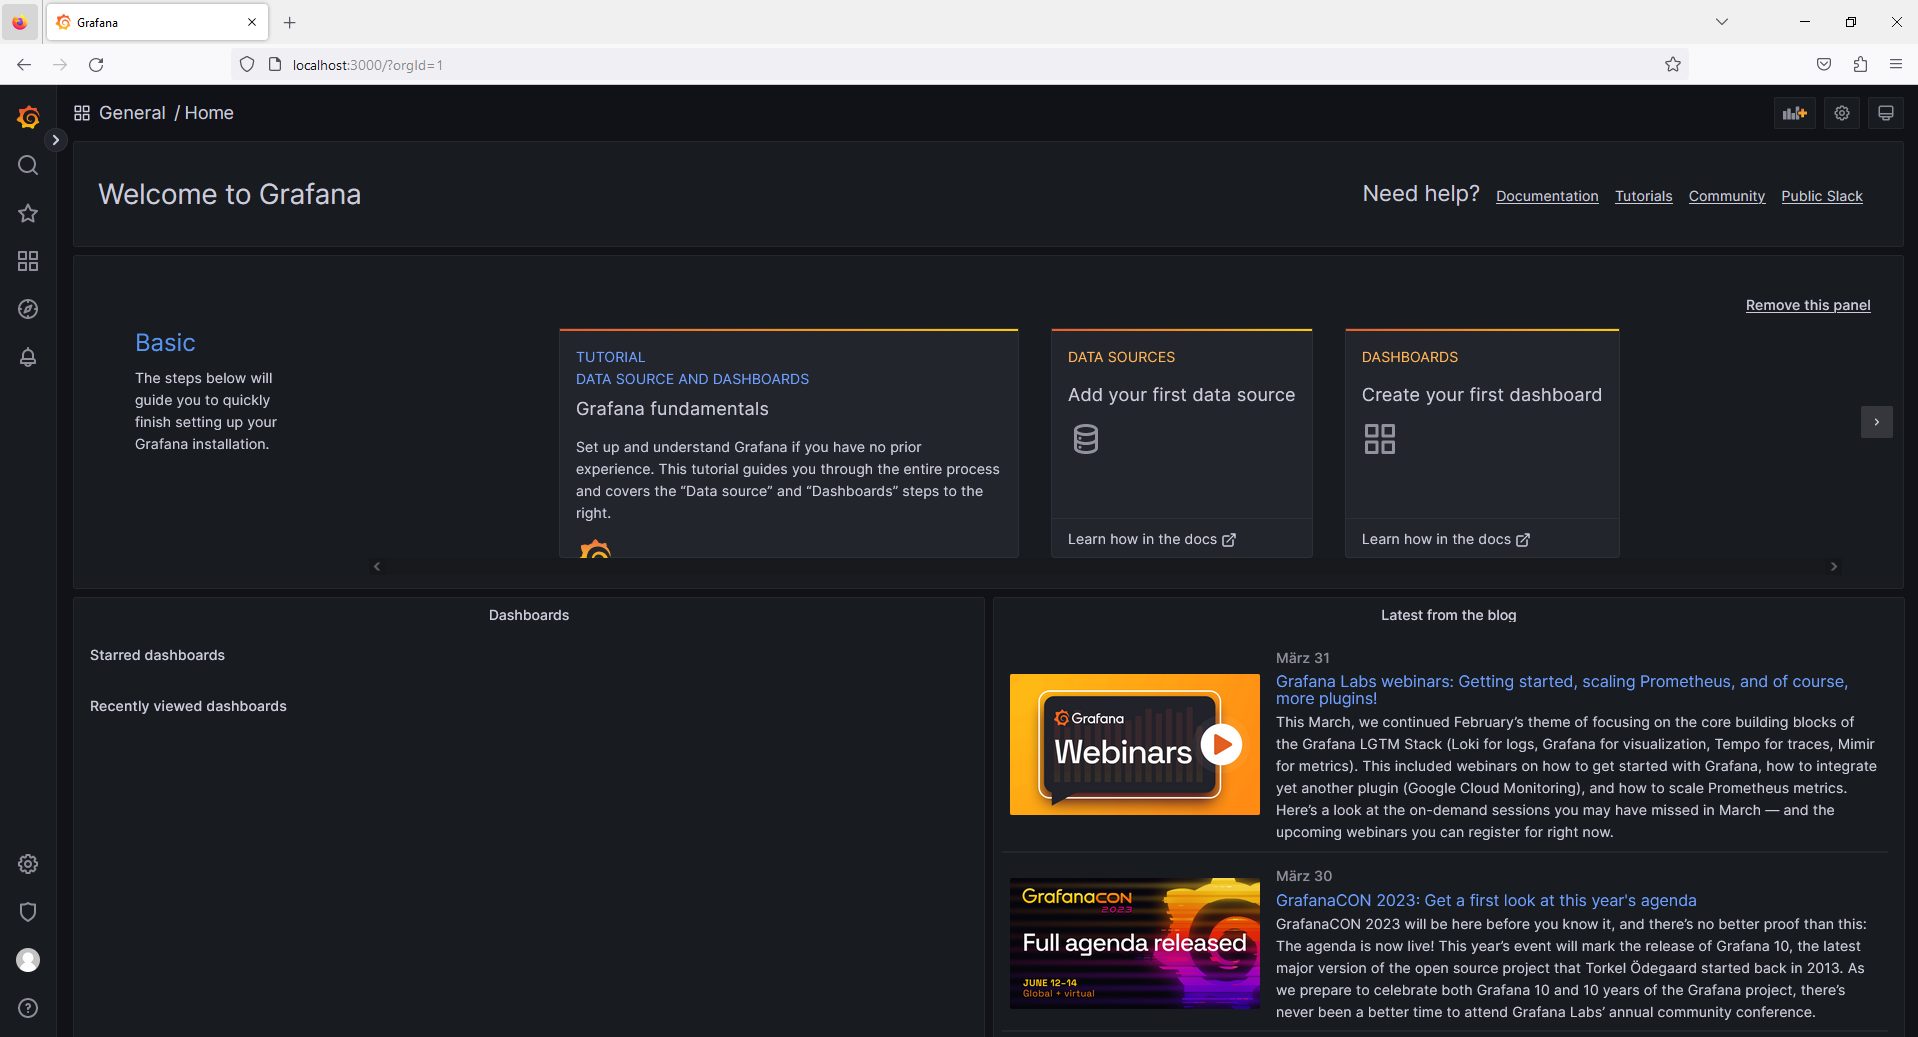
\includegraphics[width=1.5\textwidth]{assets/Installation_Grafana.png}}
        %\includegraphics[width=1.2\textwidth]{assets/5.4.2_1_Abb.jpeg}
        \caption[Screenshot der Willkommensseite von Grafana Loki]
        {Screenshot der Willkommensseite von Grafana Loki\\Quelle: Eigene Quelle und \citep{Grafana_Logs}}
        \label{fig:grafana_welcome}
        \centering
    \end{figure} 
\end{landscape}
\restoregeometry  

\subsubsection{Weiterleitung der Logdateien zu Grafana}
Grafana Loki bietet interne und externe Möglichkeiten Logdateien zu empfangen. Die internen beziehen sich auf Grafana Tools, während die externen unabhängige Methode von Grafana benutzen:

\begin{enumerate}[noitemsep]
   \item \textbf{interne Methode}:
   \begin{enumerate}[noitemsep]
      \item Promtail 
      \item Grafana Agents
   \end{enumerate}
   \item \textbf{externe Methode}
   \begin{enumerate}[noitemsep]
      \item \glsfirst{API}
      \item \gls{opentelemetry} 
   \end{enumerate}
\end{enumerate}

In unserer Arbeit verwenden wir \textbf{Promtail}, der in einem \gls{container} läuft. Diese Instanz sendet die von uns ausgewählten Logdateien an Grafana und verarbeitet alle Dateien innerhalb eines sogenannten \quotes{jobs}. Promtail kann Logdatein nur zu Grafana Loki oder zu anderen Promtail-Instanz schicken \citep{Grafana_Promtail}. Die folgende Abbildung, \ref{fig:Promtail_Diagramm}, zeigt die \glsplural{Endpoint} (links), wo Promtail installiert ist. Jeder Instanz von Promtail schickt Logdateien zu Loki (mitte), wo die Daten dann in Grafana (rechts) dargestellt werden.

%Bei verschiedenen wird jeder Typ einem eigenen \quotes{job} zugewiesen \citep{Grafana_CollectLogs}. Jeder \quotes{job} hat seine eigenen Regeln, um nach gefilterten Informationen zu suchen. 

\begin{figure}[H]
   \centering
   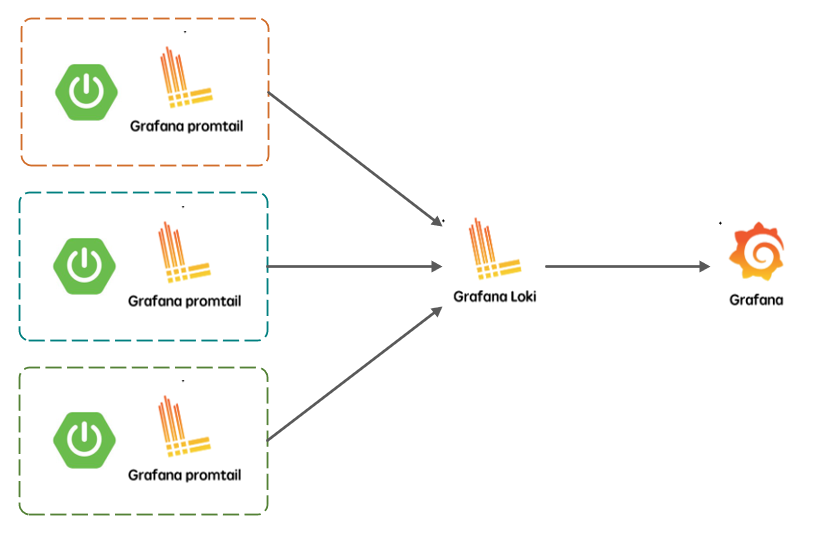
\includegraphics[width=0.6\textwidth]{assets/Promtail_Diagramm.png}
   \caption[Promtail in jeden \glsplural{Endpoint} kommuniziert sich mit Grafana Loki]
   {Promtail in jeden \glsplural{Endpoint} kommuniziert sich mit Grafana Loki\\Quelle: \citep{SpringCloud_Promtail}}
   \label{fig:Promtail_Diagramm}
   \centering
\end{figure}

In einer produktiven Umgebung ist die Installation von \textbf{Grafana Agents} auf jedem \gls{Endpoint} eine andere Lösung, um Grafana Loki mit Logdateien zu füllen. Während Promtail Logdatei nur zu Loki schickt, kann Grafana Agents Logdateien zu \gls{prometheus}, OpenTelemetry und zu Tools von \gls{GrafanaSystem}, wie \gls{mimir}, \gls{tempo}, \gls{phlare}, Loki und Grafana \citep{Grafana_Agents}. Die nächste Abbildung, \ref{fig:GrafAgents}, zeigt den Kommunikationfluss zwischen Grafana Agents und die integrieten Tools:

\begin{figure}[H]
   \centering
   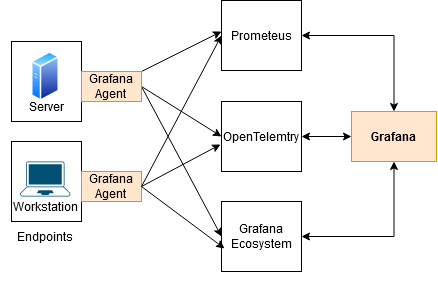
\includegraphics[width=0.6\textwidth]{assets/GrafanaAgents.drawio.png}
   \caption[Kommunikation zwischen Grafana Agents, \gls{prometheus}, OpenTelemetry und \gls{GrafanaSystem}]
   {Kommunikation zwischen Grafana Agents, \gls{prometheus}, OpenTelemetry und \gls{GrafanaSystem}\\Quelle: \citep{Grafana_Agents}}
   \label{fig:GrafAgents}
   \centering
\end{figure}

Der Kommunikationsfluss bei Grafana Agents funktioniert ähnlich, wie bei Promtail. Die \glsplural{Endpoint} (links), wo die Agents installiert sind, schicken die Logdateien zu den kompatiblen Tools (mitte), die sich wiederum mit Grafana (rechts) kommunizieren.

Die Sendung des Inhalts der Logdateien findet auch mithilfe von Grafana Loki \gls{http} \textbf{\gls{API}} statt. In diesem Fall werden die Zeile der Logdateien und nicht der Datei zum \gls{Endpoint} von Loki mit \gls{http} POST-Anfrage geschickt. 

Grafana Loki bietet auch eine Integration mit dem Open-Source-Tool \gls{opentelemetry} an, um Logdateien zu empfangen \citep{Grafana_opentelemetry}. Die Integration mit Grafana Loki erfolgt über die Nutzung von \glsplural{API}. Der \textit{Collector} läuft in derselben Umgebung wie Grafana Loki, damit er die Logdateien empfangen und verarbeiten kann. Die \textit{Agents} laufen auf jedem Endpunkt und kommunizieren mit dem \textit{Collector}. Die folgende Abbildung stellt das Kommunikationsverfahren zwischen \gls{opentelemetry} und Grafana Liki:

\begin{figure}[H]
   \centering
   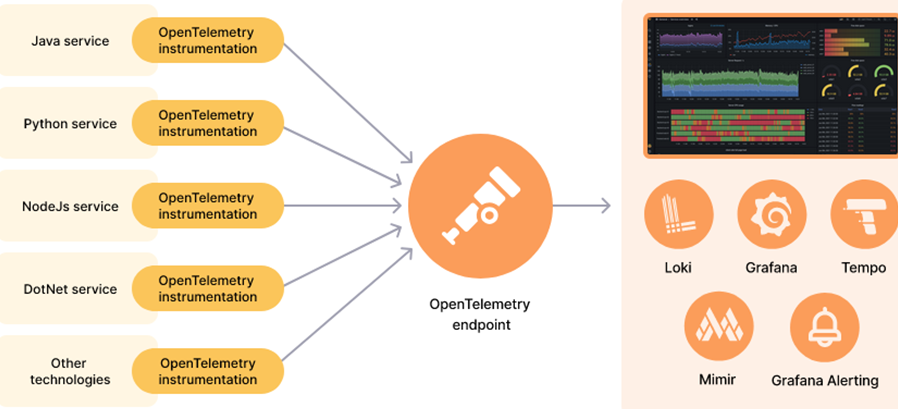
\includegraphics[width=0.8\textwidth]{assets/Grafana_OpenTelemtry.png}
   \caption[Datenfluss zwischen \gls{opentelemetry} und die Tools von \gls{GrafanaSystem}]
   {Datenfluss zwischen \gls{opentelemetry} und\gls{GrafanaSystem}\\Quelle: \citep{Grafana_WhatOpentelemetry}}
   \label{fig:UsingOpenTelemetry}
   \centering
\end{figure}

Auf der linken Seite der Abbildung \ref{fig:UsingOpenTelemetry} haben wir die verschiedenen \glsplural{Endpoint}, auf denen jeweils ein \textit{Agent} läuft. In der Mitte ist der \textit{Collector}, der die Logdateien schließlich an die Tools von \gls{GrafanaSystem} weiterleitet.

\newpage
\subsection{Aufbau der Erkennungsregel für den ausgewählten Angriff}
Ein \gls{bruteforce} lässt sich durch eine hohe Anzahl der fehlgeschlagenen Anmeldeversuche erkennen \citep{Selvaganesh_SplunkBruteForce}. Wir betrachten eine Situation, in der keine Gegenmaßnahmen wie Kontosperre nach \textit{n} beliebigen Versuchen oder \gls{mfa}, implementiert sind. Das folgende Abbildung, \ref{fig:Aktivitaetsdiagramm_Anmeldung}, stellt Diagramm mit einem allgemeinen Ablauf eines Anmeldungsverfahrens dar:

\begin{figure}[H]
   \centering
   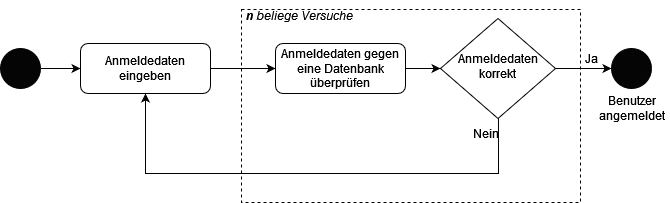
\includegraphics[width=0.8\textwidth]{assets/Anmeldeverfahren.drawio.png}
   \caption[Allgemeiner Ablauf eines Anmeldungsverfahrens]
   {Allgemeiner Ablauf eines Anmeldungsverfahrens \\Quelle: Eigene Quelle und \citep{Selvaganesh_SplunkBruteForce}}
   \label{fig:Aktivitaetsdiagramm_Anmeldung}
   \centering
\end{figure}

Grafana bietet ein Konfigurationsmuster für die Eingabe und Darstellung von \gls{ssh} Eventds an. In dieser Konfiguration sind bereits Regesätze für die 
Verarbeirtung der Log-Einträge in Loki und Quellcode für die Generierung von Grafik in Grafana. Diese Konfigurationsdatei ermöglicht eine umfassende Analyse dieser Daten \citep{VoidQuark_sshlogs}. Die gesentet Logdateien werden mithilfe der folgenden Elemente gelesen und verarbeitet:

% % \begin{table}[H]
% %    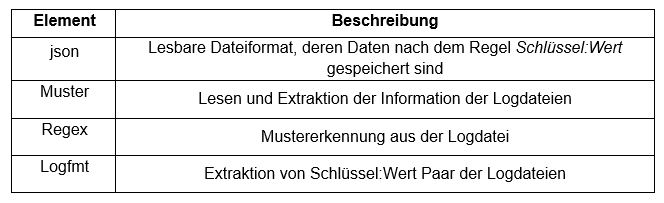
\includegraphics[width=\linewidth]{assets/tabelle_sshgrafana.png}
% %    \caption[Elementen eines Regelsätzes in Grafana Loki]
% %    {Elementen eines Regelsätzes in Grafana Loki \\Quelle: Eigene Quelle, \citep{VoidQuark_sshlogs} und \citep{Setter_Logfmt}}
% % \end{table}


\begin{table}[H]
   \setstretch{1.2}
   \begin{tabularx}{\textwidth}{|c|X|}
   \hline
   \multicolumn{1}{|c|}{\textbf{Element}} & \multicolumn{1}{|c|}{\textbf{Beschreibung}} \\
   \hline
      json & Lesbare Dateiformat, deren Daten nach dem Regel Schlüssel:Wert gespeichert sind \\
   \hline
      Muster & Lesen und Extraktion der Information der Logdateien \\
   \hline
      \glsfirst{RegExp} & Mustererkennung aus der Logdatei \\
   \hline
      Logfmt & Extraktion von Schlüssel:Wert Paar der Logdateien \\
   \hline
   \end{tabularx}
   \caption[Elementen eines Regelsätzes in Grafana Loki]
   {Elementen eines Regelsätzes in Grafana Loki \\Quelle: Eigene Quelle, \citep{VoidQuark_sshlogs} und \citep{Setter_Logfmt}}
\end{table}


%https://grafana.com/docs/loki/latest/fundamentals/labels/
%https://prometheus.io/docs/concepts/jobs_instances/

Für jedes Angriffszenario benutzen wir spezifische Regeln, die mit \gls{logql} aufgebaut sind. Die Filterung findet mithilfe von zweil Labels \quotes{instance} und \quotes{job} statt. In Promtail wird jeder \gls{Endpoint} als \quotes{Instance} bezeichnet. Eine oder mehrere \quotes{instances} werden einem \quotes{job} zugewiesen. \quotes{jobs} beziehen sich auf die Bearbeitung der Logdateien nach dem spezifizieren Regeln, in unserem Fall, Überprüfung von \gls{ssh}-Logdateien. Diese Struktur stammt aus dem Tool \gls{prometheus}. Alle unsere \quotes{instance} werden in einem \quotes{job} eingepackt, wo sie nach den gleichen Regeln verarbeitet. Zusätliche Labels können auch definiert werde \citep{Prometheus_JobInstance}. Das folgende Diagramm, \ref{fig:Labels_GrafanaLoki}, stellt die Beziehung zwischen dieser beiden Labels dar:

\begin{figure}[H]
   \centering
   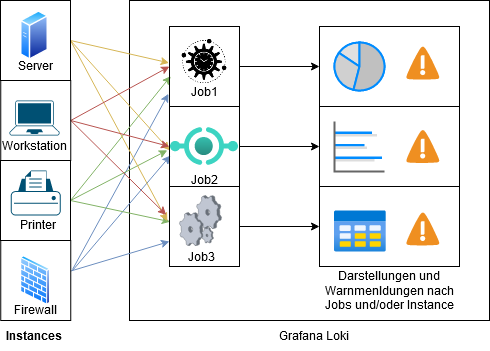
\includegraphics[width=0.8\textwidth]{assets/Instance_Jobs.drawio.png}
   \caption[Beziehung zwischen \quotes{instance} und \quotes{job}]
   {Beziehung zwischen \quotes{instance} und \quotes{job}}
   \label{fig:Labels_GrafanaLoki}
   \centering
\end{figure}

\newpage
Der Inhalt Logdateien kann dann in Grafana nach dem definierten Labels aufgerufen werden, wie auf der folgenden Abbildung \ref{fig:screenshot_labels} dargestellt:

\begin{figure}[H]
   \centering
   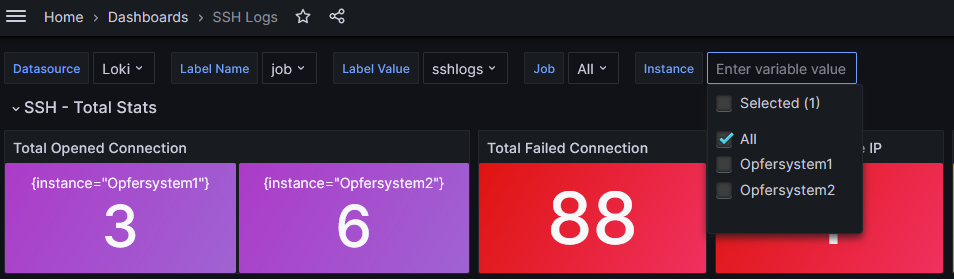
\includegraphics[width=0.7\textwidth]{assets/Grafana_labels.png}
   \caption[Aufrufe des Inhalts der Logdateien nach bestimmten Labels]
   {Aufrufe des Inhalts der Logdateien nach bestimmten Labels}
   \label{fig:screenshot_labels}
   \centering
\end{figure}

Mit \gls{logql} können auch Filterung verwendet, um nach bestimmten \quotes{instance} und/oder \quotes{jobs} die Daten aufzurufen, wie auf der Abbildung \ref{fig:screenshot_logql} dargestellt:

\begin{figure}[H]
   \centering
   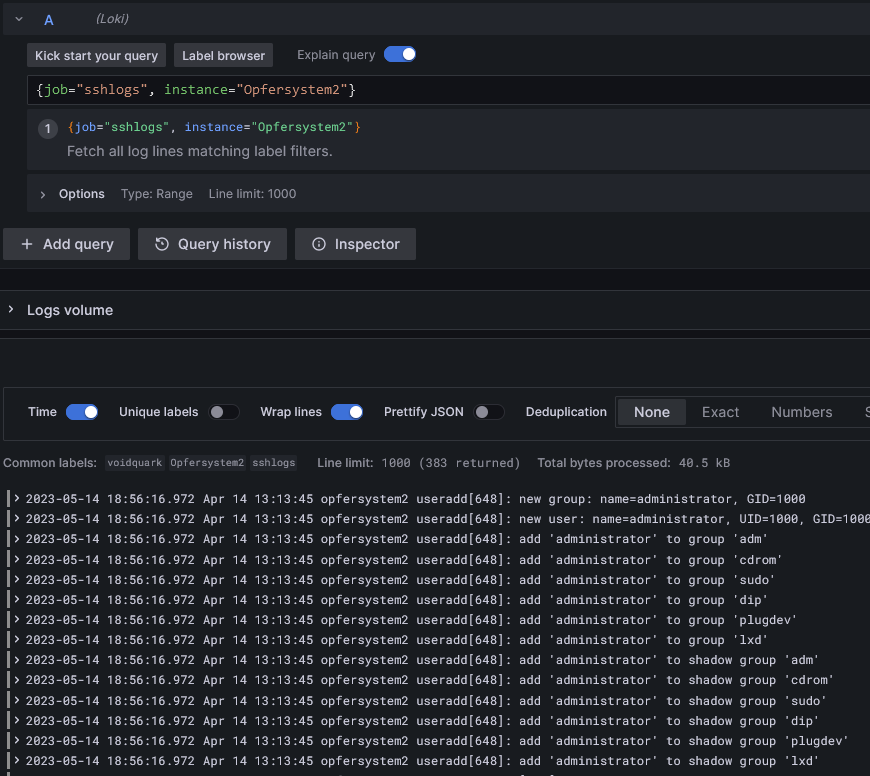
\includegraphics[width=0.7\textwidth]{assets/Logql_labels.png}
   \caption[Aufrufe des Inhalts der Logdateien mit \gls{logql}]
   {Aufrufe des Inhalts der Logdateien \gls{logql}}
   \label{fig:screenshot_logql}
   \centering
\end{figure}

In dem nächsten Abschnitt beschreiben wir, wie diese Regel in \gls{logql} geschrieben werden.

\newpage
\subsubsection{Regelsätze in LogQL}
In diesem Abschnitt fassen wir zusammen, wie eine Abfrage in \gls{logql} für eine Logdatei mit \gls{ssh} Einträgen aussieht. Für ausführliche Informationen über den Aufbau der Abfrage verweisen wir die offizielle Dokumentation, auf die diese Erklärung basiert ist \citep{Grafana_logql}. Unsere Logdatei enthält unter anderem folgende Zeile:

{\setstretch{1.0}
\begin{Verbatim}[frame=single]
14 14:05:30 opfersystem2 sshd[1698]: Failed password for administrator 
from 10.0.2.15 port 58036 ssh2
\end{Verbatim}
}

Um fehlgeschlagene Anmeldeversuche zu erkennen, extrahieren wir folgende Felder aus den \gls{ssh}-Logdateien. Diese Information verwenden wir um gleiche Events zu erkennen und deren Anzhal festzustellen. 

{\setstretch{1.0}
\begin{Verbatim}[commandchars=\\\{\},frame=single]
14 14:05:30 opfersystem2 \textbf{\textcolor{red}{sshd[}}1698]: \textbf{\textcolor{red}{Failed}} password for \textbf{\textcolor{blue}{administrator}}
from \textbf{\textcolor{blue}{10.0.2.15}} port 58036 ssh2
\end{Verbatim}
}

Wir teilen die Abfrage unten mit, um ihre Bestandteile besser zu verstehen: 

\begin{table}[H]
   \setstretch{1.2}
   \begin{tabularx}{\textwidth}{|m{5cm}|X|}
   \hline
   \multicolumn{1}{|c|}{\textbf{Element}} & \multicolumn{1}{|c|}{\textbf{Beschreibung}} \\
   \hline
   \centering
   sum by(add)
   (rate(\{job=\verb|"|\textit{JOBNAME}\verb|"|
   instance=~\verb|"|\$instance\verb|"|\} 

   & Hiermit wird die Aufsummierung der Benutzernamen definiert, die wir mit \quotes{Patterns} in \gls{logql} definiert haben. \quotes{Patterns} ermöglichen die einfache Extrahierung von Informationen aus einer Zeile. Wir holen alle Log-Einträge, die sich auf den von uns definierten Job beziehen. Wir können auch nach spezifischen Endpoint filtern, indem wir das Schlüsselwort \quotes{instance} benutzen. \\
   \hline
   \centering
   | 
   & \quotes{|} funktioniert in \gls{logql} wie eine Pipeline für die Verkettung von mehreren Suchmustern. \\
   \hline
   \centering
         |= \lq \textbf{\textcolor{red}{sshd}}[\rq 
      \\ |= \lq: \textbf{\textcolor{red}{Failed}}\rq 
    & 
    Suche nach Zeilen mit den in den rot markierten Einträgen. \\
   \hline
   \end{tabularx}
\end{table}

\begin{table}[H]
   \setstretch{1.2}
   \begin{tabularx}{\textwidth}{|m{5cm}|X|}
   \hline
   \multicolumn{1}{|c|}{\textbf{Element}} & \multicolumn{1}{|c|}{\textbf{Beschreibung}} \\
   \hline
   \centering
      !\verb|~| \lq \textbf{\textcolor{red}{invalid user}}\rq \\
      !\verb|~| \lq \textbf{\textcolor{red}{Legitimer\_Nutzer}}\rq \\
      !\verb|~| \lq \textbf{\textcolor{red}{Legitime\_Adresse}}\rq 
   & Suche nach Zeilen \textbf{ohne} diese Einträge. Wir können beispielsweise Einträge ausschließen, die auf legitimen Nutzer oder IP-Adresse beziehen, um falsche Positive zu vermeiden \\
   \hline
   \centering
      | pattern \lq<\_> for \\
      <\textbf{\textcolor{blue}{Benutzername}}> from \\
      <\textbf{\textcolor{blue}{Quelladresse}}> port <\_>\rq \\
      \verb|[|\$ \verb|__|range\verb|]|\verb|))| 
      
   & Die Definition der Wörter \quotes{Benutzername}, \quotes{Quelladresse} und als \quotes{Patterns} dienen dazu, einen Benutzernamen und eine Quelle IP-Adresse aus der Logdatei zu extrahieren. Die Platzhalter \quotes{<\_>} sind unbenannte Elemente, die in diesem Fall auf die Einträge \quotes{password} und \gls{port} in der Zeile verweisen. \\
   \hline
   \end{tabularx}
   \caption[Elementen eines Regelsätzes in Grafana Loki]
   {Elementen eines Regelsätzes in Grafana Loki \\Quelle: Eigene Quelle, \citep{VoidQuark_sshlogs} und \citep{Setter_Logfmt}}
\end{table}


% \begin{table}[H]
%    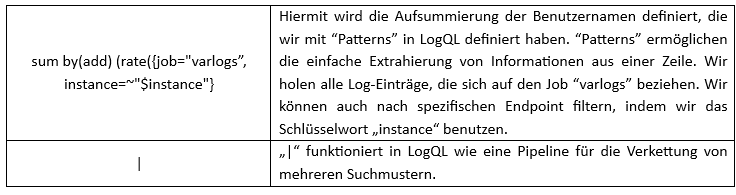
\includegraphics[width=1\linewidth]{assets/tabelle_logql_1.png}
% \end{table}

% \begin{table}[H]
%    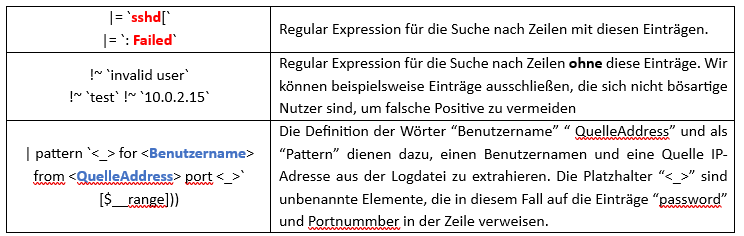
\includegraphics[width=1\linewidth]{assets/tabelle_logql_2.png}
%    \caption[Aufbau der Regelsätze in Grafana Loki für \gls{ssh} Logdateien]
%    {Aufbau der Regelsätze in Grafana Loki für \gls{ssh} Logdateien \\Quelle: Eigene Quelle, \citep{VoidQuark_sshlogs} und \citep{Grafana_logql}}
% \end{table}

Schließlich sieht der Regelsatz so aus:

{\setstretch{1.0}
\begin{Verbatim}[fontsize=\small, commandchars=\\\{\}, frame=single]
sum by(add) (rate({job="\textit{JOBNAME}", instance=~"$instance"} |= '\textbf{\textcolor{red}{sshd}}[' |= ': 
\textbf{\textcolor{red}{Failed}}' !~ '\textbf{\textcolor{red}{invalid user}}' !~ '\textbf{\textcolor{red}{Legitimer_Nutzer}}' !~ '\textbf{\textcolor{red}{Legitime_Adresse}}' |
pattern '<_> for <\textbf{\textcolor{blue}{Benutzername}}> from  <\textbf{\textcolor{blue}{Quelladresse}}> port <_>' [$__range]))
\end{Verbatim}
}

%sum by(add) (rate({job="JOBNAME", instance=~"$instance"} |= 'sshd[' |= ': Failed' !~ 'invalid user' !~ 'Legitimer_Nutzer' !~ 'Legitime_Adresse' | pattern '<_> for <Benutzername> from <Quelladresse> port <_>' [$__range]))

% \begin{table}[H]
%    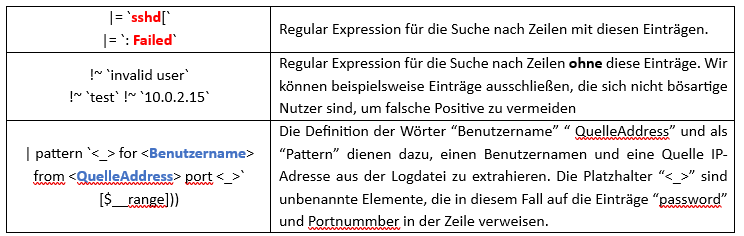
\includegraphics[width=1\linewidth]{assets/tabelle_logql_2.png}
%    \caption[Aufbau der Regelsätze in Grafana Loki für \gls{ssh} Logdateien]
%    {Aufbau der Regelsätze in Grafana Loki für \gls{ssh} Logdateien \\Quelle: Eigene Quelle, \citep{VoidQuark_sshlogs} und \citep{Grafana_logql}}
% \end{table}


\textbf{\textcolor{red}{Das sollte verbessert werden}}
Eine allgemeine Erkennungsregel in \gls{logql} würde so aussehen:
{\setstretch{1.0}
\begin{Verbatim}[frame=single]
# Gefundene Werte in den Logdateien
# Av = Anzahl fehlgeschlagener Anmeldungsversuche
# Ia = Intervallzeit zwischen fehlgeschlagenen Anmeldungsversuchen

# Festgelegte Werte für legitime und bösartige Verbindungen
# Ga = Grenze zwischen legitimen und bösartigen Anmeldungsversuchen
# Nt = Intervallzeit zwischen legitimen Anmeldungsversuchen

wenn (Av >= Ga) und (Ia < Nt)
   Warnmeldung(Brutefoce)
sonst
   weiterBeobachten()
\end{Verbatim}
}

\subsection{Hinzufügen der Regelsätze Grafana Loki}
Die Regelsätze in Grafana Loki können sowohl \textbf{manuell} im Menü \quotes{Code} als auch über die \textbf{\gls{GUI}} im Menü \quotes{Builder} geschrieben werden. Letzteres bietet eine benutzerfreundlichere Umgebung, um die Regeln zu schreiben. Die folgenden Abbildungen, \ref{fig:Loki_Code} und \ref{fig:Loki_Builder}, zeigen diese beiden Optionen:

\begin{figure}[H]
   \centering
   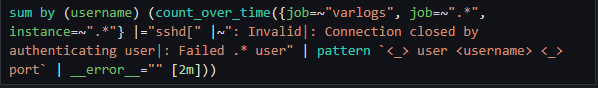
\includegraphics[width=0.85\textwidth]{assets/manuellerCodeLoki.png}
   \caption[\quotes{Code} in Grafana Loki für manuelle die Eingabe des \gls{logql}-Codes]
   {\quotes{Code} in Grafana Loki für manuelle die Eingabe des \gls{logql}-Codes. \\ Quelle: \citep{VoidQuark_sshlogs}}
   \label{fig:Loki_Code}
   \centering
\end{figure}

\begin{figure}[H]
   \centering
   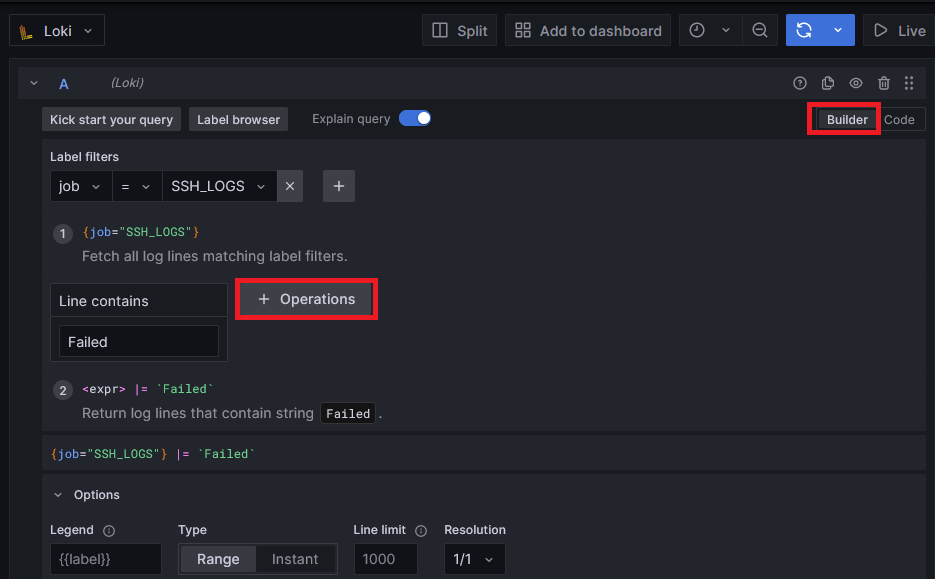
\includegraphics[width=0.85\textwidth]{assets/klickibuntyGrafana.png}
   \caption[\quotes{Builder} in Grafana Loki für nutzerfreundlichere Eingabe des \gls{logql}-Codes.]
   {\quotes{Builder} in Grafana Loki für nutzerfreundlichere Eingabe des \gls{logql}-Codes. Quelle: \citep{VoidQuark_sshlogs}}
   \label{fig:Loki_Builder}
   \centering
\end{figure}

\newpage
Beide Optionen bieten die Möglichkeit, eine Erklärung zur Abfrage anzuzeigen, wie auf der Abbildung \ref{fig:Loki_CodeInformation} gezeigt wird:
\begin{figure}[H]
   \centering
   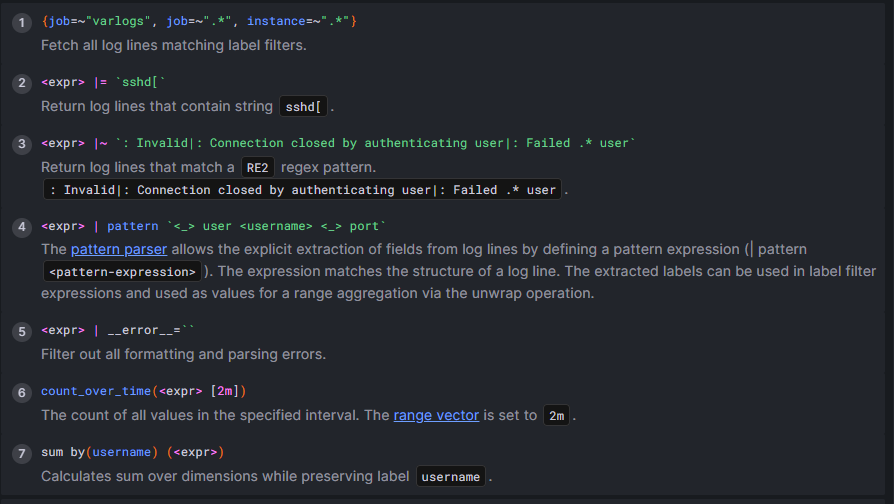
\includegraphics[width=1\textwidth]{assets/erklaerungLoki.png}
   \caption[Ausführliche Information über die Abfrage]
   {Ausführliche Information über die Abfrage\\Quelle: \citep{Grafana_QueryEditor}}
   \label{fig:Loki_CodeInformation}
   \centering
\end{figure}

Mit der Nutzung von \gls{API} ist auch möglich Regelsätze hinzufügen:
\textcolor{red}{\textbf{TODO Citar regra API https://grafana.com/docs/loki/latest/api/}}

\newpage
\newgeometry{right=30mm, left=30mm} 
\thispagestyle{lscape}
\begin{landscape}
   Nachdem die \gls{ssh}-Logdateien gelesen und verarbeitet wurden, bekommen wir von Grafana Loki die zusammenfassende Ergebnissen, wie unter auf der Abbildung \ref{fig:Grafana_DetailedStats} dargestellt:
    \begin{figure}[H]
       % \centering
        \centerline{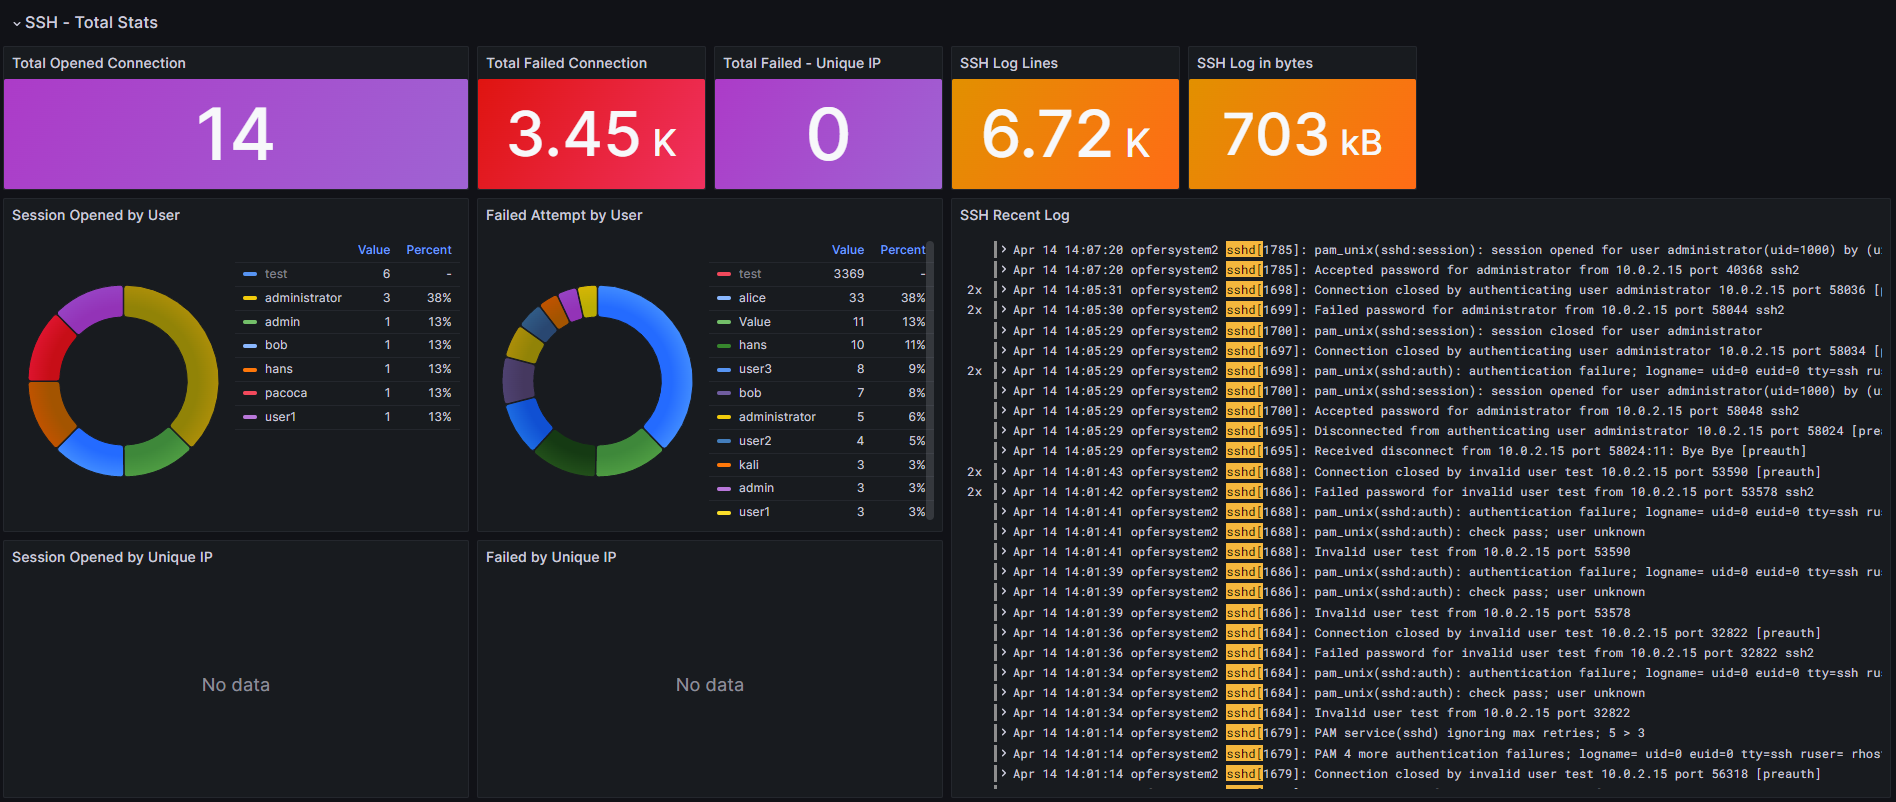
\includegraphics[width=1.7\textwidth]{assets/GrafanaLoki_ssh}}
        %\includegraphics[width=1.2\textwidth]{assets/5.4.2_1_Abb.jpeg}
        \caption[Ausgabe der Verarbeitung der \gls{ssh} Logdateien von Grafana Loki]
        {Ausgabe der Verarbeitung der \gls{ssh} Logdateien von Grafana Loki}
        \label{fig:Grafana_Grafik}
        \centering
    \end{figure} 
\end{landscape}
\restoregeometry

\newpage
\newgeometry{right=30mm, left=30mm} 
\thispagestyle{lscape}
\begin{landscape}
   Das nächste Abbidung, \ref{fig:Grafana_DetailedStats}, gibt ausführliche Informationen der Logdateien:
    \begin{figure}[H]
       % \centering
        \centerline{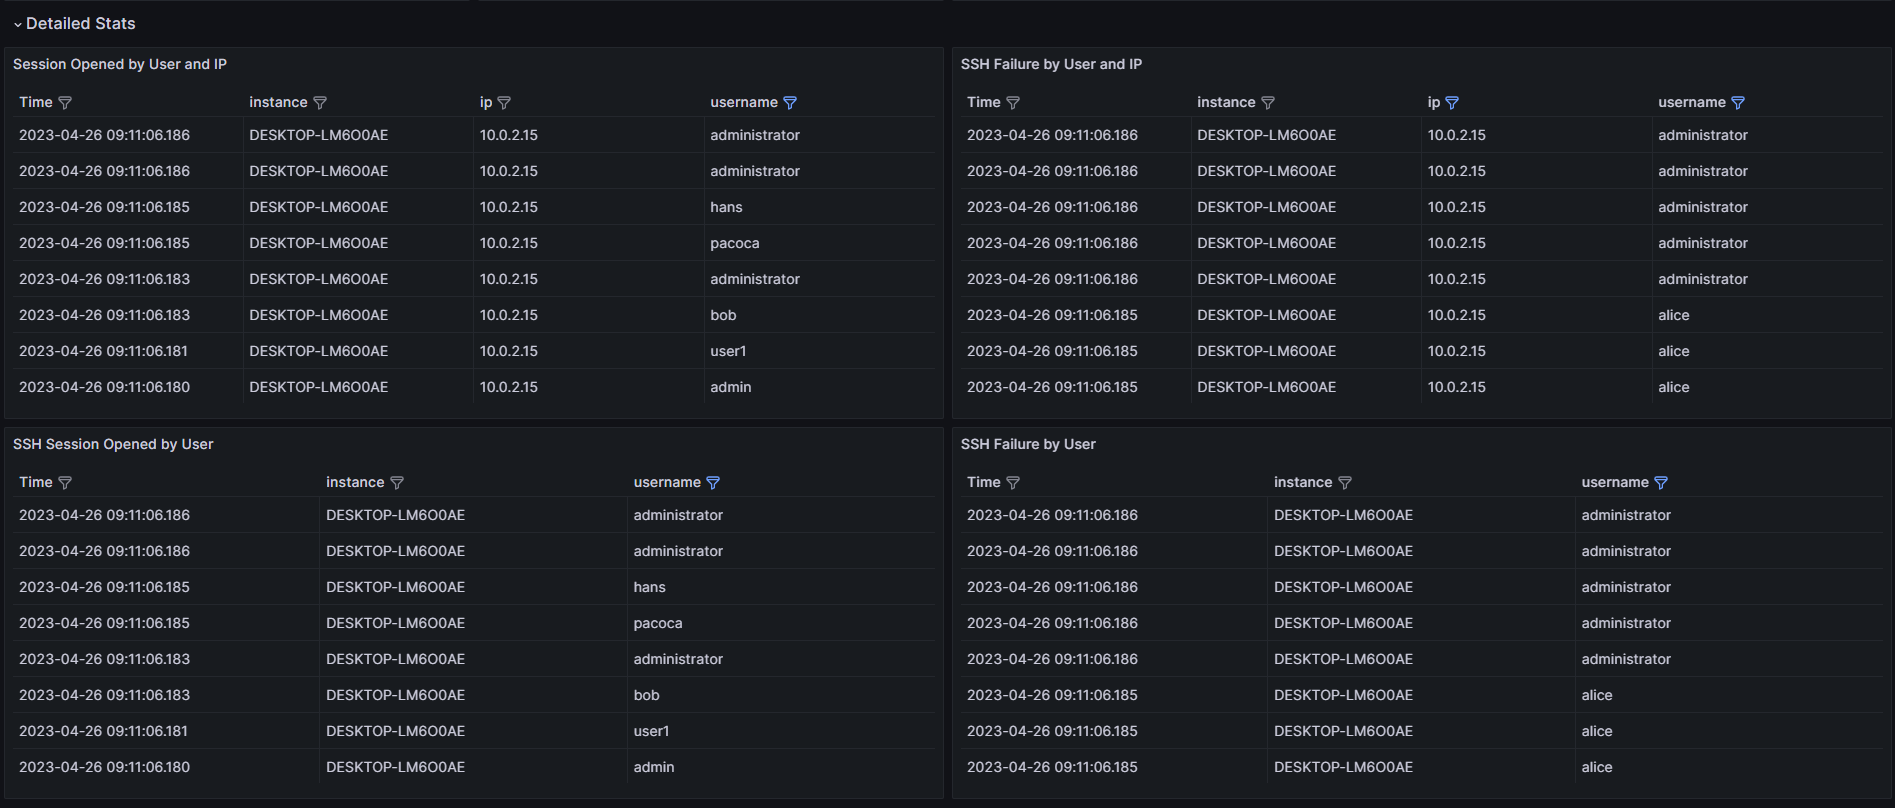
\includegraphics[width=1.7\textwidth]{assets/GrafanaLoki_sshDetailed.png}}
        \caption[Ausführliche Darstellung der \gls{ssh} Logdateien von Grafana Loki]
        {Ausführliche Darstellung der \gls{ssh} Logdateien von Grafana Loki}
        \label{fig:Grafana_DetailedStats}
        \centering
    \end{figure} 
\end{landscape}
\restoregeometry

% \thispagestyle{lscape}
% \begin{landscape}
%    Das nächste Bild gibt ausführliche Informationen der Logdateien:
%    \begin{center}
%       \begin{figure}[H]
%          \centering
%          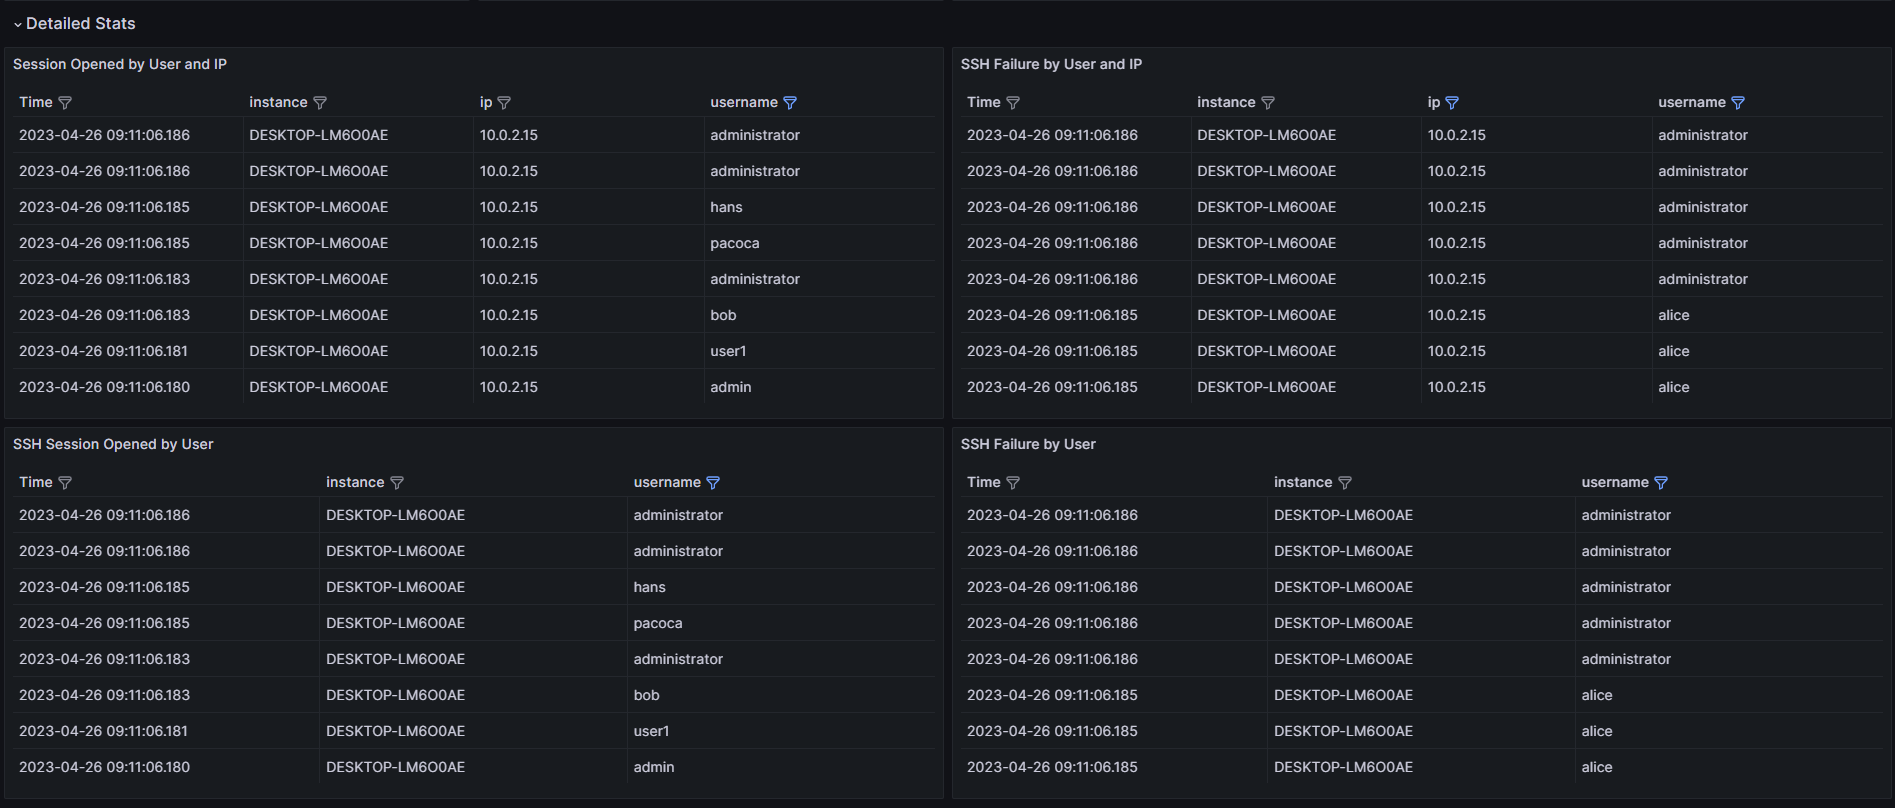
\includegraphics[width=1.3\textwidth]{assets/GrafanaLoki_sshDetailed.png}.
%          \caption[Ausführliche Darstellung der \gls{ssh} Logdateien von Grafana Loki]
%          {Ausführliche Darstellung der \gls{ssh} Logdateien von Grafana Loki\\Quelle: Eigene Quelle and \citep{VoidQuark_sshlogs}}
%          \centering
%       \end{figure}
%    \end{center}
% \end{landscape}

\subsection{Einrichtung der Warnmeldungen in Grafana}
In den vorherigen Teilen dieser Arbeit haben wir uns damit auseinandergesetzt, Grafana so einzurichten, dass wir schließlich eine Lösung ähnlich einer \gls{SIEM} erhalten. Von unseren ursprünglichen Ziele haben wir bereits Folgendes erreicht:

{\setstretch{1}
\begin{enumerate}[noitemsep]
   \item	Sammlung der Logdateien von den \glsplural{Endpoint} mit Promtail
   \item Anpassung der Logdateien für die Weiterleitung an Grafana Loki
   \item Nutzung von Regelsätzen in Loki für die Analysierung der \gls{ssh} Logdateien
   \item Graphische Darstellung der Ergebnissen in Grafana mit den in Loki verwendeten Regelsätzen
\end{enumerate}
}

Unser letztes Ziel besteht darin, Warnmeldungen für potenzielle Angriffe mithilfe der Ergebnisse von Loki zu generieren. Grafana kann sowohl intern mit der Funktionalität \quotes{Alerting} als auch extern mit \glsplural{plugin}, wie \textbf{Alertmanager}, Warnmeldungen generieren. Der zweite kann Daten von \gls{prometheus}, \gls{cortex} und \gls{mimir} als Datenquelle verwenden \citep{Grafana_Alertmanager} und kann Daten von beliebigen \glsplural{Endpoint} empfangen. Die Regelsätze des Alertmanagers haben folgendes Muster:

{\setstretch{1.0}
\begin{Verbatim}[frame=single]
# Warnmeldungen können in beliebigen Gruppen kategorisiert werden. Diese
können von den Nutzern entsprechend ihrer Anforderungen und Bedürfnisse 
definiert werden.
groups:
      # Ab diesem Punkt beginnen wir mit der Definition der Regelsätze 
      für die Erkennung von Warnmeldungen. Diese umfassen:
   - name: example
     rules:
    - alert: HighRequestLatency

      # LogQL-Regelsätze für die Erkennung der Warnmeldung, welche die 
      in den vorherigen Schritten definierten Abfragen verwenden.
      expr: job:request_latency_seconds:mean5m{job="SSH_LOGS"} > 0.5
      for: 10m
       labels:
         severity: page
       annotations:
         summary: High request latency
\end{Verbatim}
}

%verbatim comments
%lst listing

Grafana hat auch ein eigenes internes Tool, um Warnmeldungen zu konfigurieren: \textbf{Alerting}. In dieser Arbeit versuchen wir unser Warnmeldungs-System mithilfe dieses Tools aufzubauen.

Die Warnmeldungen können direkt in der \gls{GUI} von Grafana konfiguriert werden. Dazu folgt man den folgenden Schritten \citep{Grafana_alerting}:

{\setstretch{1}
\begin{enumerate}[noitemsep]
   \item Name der Regel
   \item Regelsätze in \gls{logql}
   \item Definition von Gruppen für jede Art von Warnmeldung. Gruppen können später verschiedenen Einstellungen zugewiesen werden, wie z.B. Benachrichtigungen und Inhalte.
   \item Informationen über die Warnmeldung, wie eine eindeutige ID und eine Beschreibung. Der Nutzer kann diese Felder so definieren, wie es notwendig ist.
   \item Benachrichtigung der Zielgruppe, die diesen Fall später bearbeiten wird.
   \item Labels zur besseren Organisation der Warnmeldungen.
   \item Konfiguration von E-Mail in Grafana für die Weiterleitung der Warnmeldungen.
\end{enumerate}
}

Für unseren ersten Test erstellen wir Warnmeldungen für fehlgeschlagene Anmeldeversuche. Wir haben die oben genannten Elemente definiert und die folgenden Regelsätze verwendet \citep{VoidQuark_sshlogs}:

{\setstretch{1.0}
\begin{Verbatim}[frame=single]
# (A) Anzahl von fehlgeschlagenen Anmeldeversuche für existierenden
Benutzernamen:
sum by (username) (count_over_time({$label_name=~"$label_value",
job=~"$job", instance=~"$instance"} |="sshd[" |~": Invalid|: 
Connection closed by authenticating user|: Failed .* user" | 
pattern '<_> user <username> <_> port' | __error__="" 
[$__interval]))

# (B) Anzahl von Fehlgeschlagenen Anmeldeversuche für nicht 
existierenden Benutzernamen:
sum by (username) (count_over_time({$label_name=~"$label_value", 
job=~"$job", instance=~"$instance"} |="sshd[" |=": Failed" !~"invalid 
user" | pattern '<_> for <username> from <_> port' | __error__=""
[$__interval]))

# Wenn die Anzahl von (A) oder von (B) größer als fünf ist, dann wird
die Warnmeldung als E-Mail an dem Ziel geschickt.
\end{Verbatim}
}

% discard lines with Server Ansible - https://grafana.com/docs/loki/latest/logql/log_queries/

Im Anhang \ref{appendix:Warnmedungskonfiguration} befindet sich die Konfigurationsdatei für unsere Warnmeldung.

Nachdem alles korrekt konfiguriert wurde, haben wir die folgende E-Mail erhalten:
\begin{figure}[H]
   \centering
   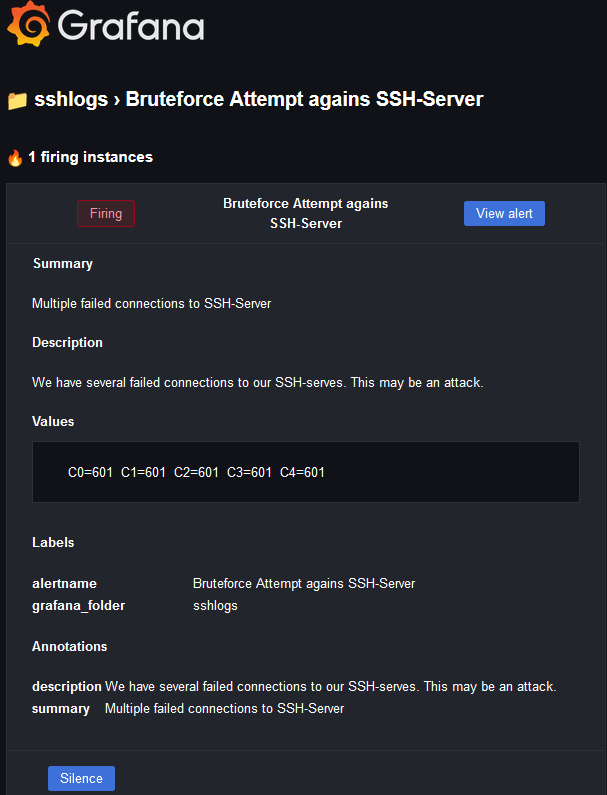
\includegraphics[width=0.7\textwidth]{assets/GrafanaWarnmeldung.png}
   \caption[E-Mail Warnmeldung von Grafana]
   {E-Mail Warnmeldung von Grafana}
   \centering
\end{figure}

%Das Alerting-Tool von Grafana bietet keine direkte Integration zu einem \gls{IDS}, \gls{IPS}, \gls{SIEM} oder einer \gls{API} an. Die Kommunikation mit solchen \glsplural{Endpoint} lässt sich jedoch mithilfe von \textbf{\gls{webhook}} konfigurieren \citep{Grafana_Notifications}.

% enabled = true
% host = smtp.gmail.com:587
% user = alertsgrafanaBA@gmail.com
% # If the password contains # or ; you have to wrap it with triple quotes. Ex """#password;"""
% password = "sexpjkbdsdwrkgqm"
  \section{Evaluation der Implementation mit echten Logdateien}


  \section{Fazit}

\subsection{Diskussion der Ergebnisse}
In dieser Arbeit emulierten wir, mithilfe von Grafana, Loki und Promtail eine \gls{SIEM}-Lösung, um Überwachungsmechanismen anhand von Logdateien zu erstellen. In der Tabelle \ref{tab:VerewendeteTools} zeigen wir die Rolle jedes verwendeten Tools bei der Erreichung unseres Ziels:

\begin{table}[h]
    \centering
    \setstretch{1.2}
    \begin{tabular}{|c|c|}
    \hline
    \textbf{Tool}    & \textbf{Funktionalität}         \\ \hline
    Promtail         & Datensammlung                   \\ \hline
    Loki             & Normalisierung und Vearbeitung  \\ \hline
    Grafana          & Berichts- und Grafikgenerierung \\ \hline
    Grafana:Alerting & Generierung von Warnmeldungen   \\ \hline
    \end{tabular}
    \caption{Verwendete Tools und ihre Hauptfunktionalitäten} 
    {Verwendete Tools und ihre Hauptfunktionalitäten}
    \label{tab:VerewendeteTools}
\end{table}

Wir stellen fest, dass die verwendeten Tools eine kosteneffektive Möglichkeit bieten, ein Überwachungssystem zu implementieren. Die Methoden zur Erkennung von Angriffen lassen sich anhand der \glsfirst{ttp} der \gls{mitre} Matrix definieren. Nach der Auswahl eines Angriffs erstellen wir Regelsätze mit der Abfragesprache \gls{logql} in Loki, um Muster zu identifizieren, die auf den ausgewählten Angriff hindeuten. Diese Regelsätze werden dann verwendet, um Warnmeldungen über den Angriff zu generieren und zu versenden.

Zu unsere initialen Ziele:

{\setstretch{1.5}
\begin{itemize}[noitemsep]
   \item Wie können wir ein Log-Analyse-Tool konfigurieren, dass es vordefinierte Angriffe nach der \gls{mitre} Matrix automatisch erkennen kann? 
   \item Wie können wir allgemeine Regelsätze definieren, sodass wir sie später für die verschiedene \gls{ttp} der \gls{mitre} Matrix anpassen können?
\end{itemize}
}

können wir sagen, dass die \gls{mitre} Matrix umfangreiche Informationen anbietet, um präzise Regelsätze zu generieren. 

\subsection{Herausforderungen}
Zu unserem primären Ziel können wir sagen, dass die \gls{mitre}-Matrix umfangreiche Informationen bietet, um zielgerichtete Regelsätze zu generieren. Die Erstellung dieser Regelsätze kann jedoch eine der größten Herausforderungen bei der Implementierung darstellen, da die Verwendung der Abfragesprache \gls{logql} viel Zeit in Anspruch nehmen kann. Sobald diese Hürde jedoch überwunden ist, ist es möglich, präzise Regelsätze zu erstellen, um potenzielle Angriffe zu identifizieren. Die Lernkurve für den Aufbau der richtigen Regelsätze kann eine große Herausforderung darstellen, wie auch in unserem Fall.

Da Logdateien aus produktiven Umgebungen eine große Menge an Informationen enthalten, müssen die Regelsätze so definiert werden, dass sie die relevanten Informationen wie IP-Adresse, Portnummer, Zeitfenster und Zeitabstände zwischen Anfragen filtern und nach Angriffsmustern kategorisieren können.

Die zweite große Herausforderung bestand darin, die richtigen Einstellungen und Funktionen von Promtail, Loki und Grafana zu verwenden. Das Beherrschen dieser Elemente kann dazu beitragen, dass die Anwendungen reibungslos funktionieren und vertrauenswürdige Ergebnisse liefern.

Die korrekte Konfigurierung von Promtail, besonders von \quotes{scrape\_configs}, begünstigt die Extrahierung spezifischer Informationen und die Generierung präziser \quotes{Labels}. Das Verständnis über die vielfältigen Funktionalitäten von Grafana trägt dazu bei, dass die ausgegebenen Daten die notwendigen Informationen enthalten, um den Entscheidungsprozess zu erleichtern. Die richtigen Einstellungen gewährleisten eine fehlerfreie Nutzung der Anwendungen und erleichtert ihre Skalierbarkeit. In diesem Fall können sowohl die offizielle Dokumentation als auch die offiziellen Forenbeiträge dazu beitragen, die Tools richtig zu konfigurieren.

\newpage
Letztendlich sind \quotes{Labels} wichtige Elemente bei Grafana, Loki und Promtail. Die richtige Indizierung spielt eine entscheidende Rolle für die Leistung der Anwendung. Die Verwendung vieler \quotes{Labels} erfordert hohe Rechenkapazität und kann auch zu fehlerhaften Ergebnissen führen. Die Rechenkapazität muss ebenfalls angepasst werden, um Abstürzen wegen steigenden Anfragen (siehe Abbildung \ref{fig:Eskalation_Labels} auf Seite \pageref{fig:Eskalation_Labels}) zu vermeiden.

\subsection{Zukünftige Forschung}
Dieser Arbeit ermöglicht eine Weiterentwicklugn in verschiedenen Bereichen:
 
\begin{itemize}[noitemsep]
    \item \textbf{Abdeckung vielen möglichen \glsplural{Cyberangriff}n mit neuen Regelsätze und Dashboards}:
\end{itemize}

Mit der Nutzung der \glsfirst{ttp} der \gls{mitre} Matrix ist es möglich, Regelsätze in \gls{logql} für andere \glsplural{Cyberangriff} aufzubauen und dadurch Logdateien aus verschiedenen Systemen und Anwendungen zu verwenden. Mit anderen Regelsätzen ist es möglich umfassende Sicherheit für produktive Umgebungen zu bieten, indem mehr \glsplural{usecases} abgedeckt werden, um Angriffe zu erkennen. Zur Unterstützung bietet Grafana in ihrer offizielen Webseite bereits kundenspezifische Dashboards an, die verwendet und an die jeweilige Situation angepasst werden können.

\begin{itemize}[noitemsep]
    \item \textbf{Beherschung der Tools: Promtail, Loki und Grafana}:
\end{itemize}

Grafana, Loki und Promtail bieten in ihrer Konfiguration verschiedenen Möglichkeiten, um Informationen von Logdateien zu extrahieren, zu filtern und zu analysieren. Eine tiefe Beherrschung von \quotes{scrape\_configs} von Promtail trägt dazu bei, Logdateien zu erkennen und wichtige Informtionen direkt zu filtern, ohne das weitere Abfragen notwendig sind, indem auch Leistung gespart wird. Eine Weiterarbeit mit der \gls{abfragesprache} \gls{logql} hilft dabei, präzise und effizieren Abfrage aufzubauen, um bessere Grafiken und/oder Warnmeldung zu genieren. Zusätzlich kann die vielfältigen Funktionalitäten von Grafana dabei unterstützen, zuverlässige Grafiken und Tabellen zu generieren, um nützliche Informationen aus den Logdateien grafisch darzustellen. Die Beherrschung dieses Tool stellt auch eine mögliche und vielversprechende weitere Recherche dar. 


\begin{itemize}[noitemsep]
    \item \textbf{Umfangreiche Beobachtbarkeit mit den Tools der \textit{\gls{GrafanaSystem}}}:
\end{itemize}

Die Tools um den \textit{\gls{GrafanaSystem}} bieten viele Möglichkeiten, um eine deutliche und akkurate Beobachtbarkeit eines Systems durchzuführen. Wenn kombiniert, ermöglichen sie eine holistische Analyse von \gls{pillarobservability}. Die kombinierte Implementierung in einer produktiven Umgebung kann dazu beitragen, die Sicherheit eines Systems auch bei skalierbaren Umgebungen zu verbessern. Eine Recherche in dieser Richtung hat auch die Möglichkeit, positive Ergebnisse zu liefern.


\begin{itemize}[noitemsep]
    \item \textbf{Automatische Antworten auf mögliche \glsplural{Cyberangriff}n}:
\end{itemize}

Eine umfangreiche \gls{SIEM}-Lösung bietet laut \cite{Mohammed_NOC} die wichtigsten Informatinen, um Angriffe zu erkennen. Die Sicherheitsanalyse stoppt jedoch nicht in der Erkennung, sondern verlangt Handlungen, um laufende Angriffe zu stoppen oder potenzielle zu verhindern. Die Entwicklung oder die Integration von existierenden Tools, um automatisch gegen \glsplural{Cyberangriff} zu handeln, stellen auch eine mögliche Perspektive für zukünftige Recherche dar.

\begin{itemize}[noitemsep]
    \item \textbf{Nutzung von \gls{KI}}:
\end{itemize}

Moderne Angriffe haben heutzutage einen dynamischen Aspekt, der sich an die Umgebung anpasst, insbesondere durch die fortschreitende Entwicklung von \glsfirst{KI} \citep{Guembe_AIHACKER}. \gls{KI} kann zur Automatisierung von Aufgaben oder zur effizienten Datenanalyse eingesetzt werden. Für die Weiterentwicklung dieser Arbeit kann \gls{KI} eine Unterstützung bei dem Aufbau von performanteren Regelsätzen bieten, um zuverlässiger und effizienter Log-Analyse zu gestalten.

Diese Möglichkeiten zusammen oder getrennt könnten dazu beitragen, einen sicheren Netzwerkverkehr zu gewährleisten.

  %\nocite{*}
  \begingroup
    \setlength{\bibsep}{4pt}
    \setstretch{1}
    \bibliography{9_Referenzen}
  \endgroup
  \bibliographystyle{apalike}
  \begin{appendices}
    \section{Originalle Einstellungsdateien}\label{appendix:orgGrafana}

\subsection{Loki}
{\setstretch{0.5}
\begin{Verbatim}[frame=single,fontsize=\small]
    auth_enabled: false

    server:
      http_listen_port: 3100
      grpc_listen_port: 9096
    
    common:
      instance_addr: 127.0.0.1
      path_prefix: /tmp/loki
      storage:
        filesystem:
          chunks_directory: /tmp/loki/chunks
          rules_directory: /tmp/loki/rules
      replication_factor: 1
      ring:
        kvstore:
          store: inmemory
    
    query_range:
      results_cache:
        cache:
          embedded_cache:
            enabled: true
            max_size_mb: 100
    
    schema_config:
      configs:
        - from: 2020-10-24
          store: boltdb-shipper
          object_store: filesystem
          schema: v11
          index:
            prefix: index_
            period: 24h
    
    ruler:
      alertmanager_url: http://localhost:9093
\end{Verbatim}
}

\subsection{Promtail}

{\setstretch{0.5}
\begin{Verbatim}[frame=single]
    server:
    http_listen_port: 9080
    grpc_listen_port: 0
  
  positions:
    filename: /tmp/positions.yaml
  
  clients:
    - url: http://loki:3100/loki/api/v1/push
  
  scrape_configs:
  - job_name: system
    static_configs:
    - targets:
        - localhost
      labels:
        job: varlogs
        __path__: /var/log/*log
  
\end{Verbatim}
}
    \section{Angepasste Einstellungsdateien von Grafana}\label{appendix:AngepasstGrafana}

Unten befindet sich die angepasste Konfigurationsdateien \citep{Polinowski_PGL}:

\begin{itemize}[noitemsep]
    \item \textbf{Loki}
\end{itemize}

{\setstretch{0.5}
\begin{Verbatim}[frame=single]
  auth_enabled: false

  server:
    http_listen_port: 3100
    grpc_listen_port: 9096
  
  ingester:
    wal:
      enabled: true
      dir: /tmp/wal
    config:
      max_block_size: 67108864
      max_uncompressed_block_size: 67108864
      chunk_size: 1048576
    lifecycler:
      address: 127.0.0.1
      ring:
        kvstore:
          store: inmemory
        replication_factor: 1
      final_sleep: 0s
    chunk_idle_period: 1h       
    # Any chunk not receiving new logs in this time will be flushed
    max_chunk_age: 1h           
    # All chunks will be flushed when they hit this age, default is 1h
    chunk_target_size: 1048576  
    # Loki will attempt to build chunks up to 1.5MB, flushing first if
    chunk_idle_period or max_chunk_age is reached first
    chunk_retain_period: 30s    
    # Must be greater than index read cache TTL if using an index cache
    (Default index read cache TTL is 5m)
    max_transfer_retries: 0    
    # Chunk transfers disabled
  
  schema_config:
    configs:
      - from: 2020-10-24
        store: boltdb-shipper
        object_store: filesystem
        schema: v11
        index:
          prefix: index_
          period: 24h
  
  storage_config:
    boltdb_shipper:
      active_index_directory: /tmp/loki/boltdb-shipper-active
      cache_location: /tmp/loki/boltdb-shipper-cache
      cache_ttl: 24h         
      # Can be increased for faster performance over longer query 
      periods, uses more disk space
      shared_store: filesystem
    filesystem:
      directory: /tmp/loki/chunks
  
  compactor:
    working_directory: /tmp/loki/boltdb-shipper-compactor
    shared_store: filesystem
  
  limits_config:
    reject_old_samples: true
    reject_old_samples_max_age: 168h
    ingestion_rate_mb: 1024
    ingestion_burst_size_mb: 1024
    ingestion_rate_strategy: local
    per_stream_rate_limit: 12MB
    max_query_series: 100000
    max_query_parallelism: 32
    split_queries_by_interval: 24h
    max_query_length: 0h
  
  querier:
    max_concurrent: 2048
  
  frontend:
    compress_responses: true
    scheduler_worker_concurrency: 20
  
  query_range:
    parallelise_shardable_queries: false
  
  table_manager:
    retention_deletes_enabled: false
    retention_period: 360s
  
  ruler:
    storage:
      type: local
      local:
        directory: /tmp/loki/rules
    rule_path: /loki/rules-temp
    alertmanager_url: http://localhost:9093
    ring:
      kvstore:
        store: inmemory
    enable_api: true
\end{Verbatim}
}

\begin{itemize}[noitemsep]
    \item \textbf{Promtail} 
\end{itemize}

{\setstretch{0.5}
\begin{Verbatim}[frame=single]
  ---
  server:
    http_listen_port: 9080
    grpc_listen_port: 0
  
  positions:
    filename: /tmp/positions.yaml
  
  clients:
    - url: http://loki:3100/loki/api/v1/push
      tenant_id: tenant1
  
  scrape_configs:
  - job_name: sshlogs
    decompression:
      enabled: true
      initial_delay: 15s
      format: gz
    static_configs:
    - targets:
        - loki
      labels:
        job: sshlogs
        #env: voidquart
        instance: Opfersystem1
        __path__: /opt/*.gz 
\end{Verbatim}
}

\newpage
\begin{itemize}[noitemsep]
    \item \textbf{Docker Compose Datei} 
\end{itemize}

{\setstretch{0.5}
\begin{Verbatim}[frame=single]
  version: "3"

  networks:
    loki:
  
  services:
    loki:
      image: grafana/loki:2.4.1
      volumes:
        -  ${PWD}/loki-config.yaml:/etc/loki/loki-config.yaml
      ports:
        - "3100:3100"
      command: -config.file=/etc/loki/local-config.yaml
      networks:
        - loki
  
    promtail:
      image: grafana/promtail:2.8.2
      container_name: Opfersystem1
      volumes:
        - ${PWD}/promtail-local-config_opfer1.yaml:/etc/promtail/promtail
        -config.yaml
        - ${PWD}/temp/:/opt/
      command: -config.file=/etc/promtail/promtail-config.yaml 
               -config.expand-env=true 
               #-querier.max-outstanding-requests-per-tenant= 2048
      networks:
        - loki
  
    grafana:
      image: grafana/grafana:latest
      ports:
        - "3000:3000"
      networks:
        - loki  
\end{Verbatim}
} 
    \section{Angepasste Einstellungsdateien von Grafana}\label{appendix:Warnmedungskonfiguration}

Unten befindet sich unser Regel für die Generierung von Warnmeldungen in Fälle eines \gls{bruteforce}s gegen \gls{ssh} Server.

{\setstretch{0.5}
\begin{Verbatim}[frame=single]
apiVersion: 1
groups:
    - orgId: 1
      name: sshTeam
      folder: sshlogs
      interval: 1m
      rules:
        - uid: lHYZTLPVz
          title: Bruteforce Attempt agains SSH-Server
          condition: C
          data:
            - refId: A
              queryType: range
              relativeTimeRange:
                from: 600
                to: 0
              datasourceUid: sx2e5YE4k
              model:
                datasource:
                    type: loki
                    uid: sx2e5YE4k
                editorMode: code
                expr: 'sum by(username) (count_over_time({job=~"varlogs", 
                job=~".*", instance=~".*"} |= `sshd[` |~ `: Invalid|: 
                Connection closed by authenticating user|: Failed .* user` 
                != `test` | pattern `<_> user <username> <_> port` | 
                __error__=`` [2400h]))'
                hide: false
                intervalMs: 1000
                maxDataPoints: 43200
                queryType: range
                refId: A
            - refId: B
              queryType: range
              relativeTimeRange:
                from: 600
                to: 0
              datasourceUid: sx2e5YE4k
              model:
                datasource:
                    type: loki
                    uid: sx2e5YE4k
                editorMode: code
                expr: 'sum by(username) (count_over_time({job=~"varlogs", 
                job=~".*", instance=~".*"} |= `sshd[` |= `: Failed` !~ 
                `invalid user` != `test` | pattern `<_> for <username> 
                from <_> port` | __error__=`` [2400h]))'
                hide: false
                intervalMs: 1000
                maxDataPoints: 43200
                queryType: range
                refId: B
            - refId: C
              datasourceUid: __expr__
              model:
                conditions:
                    - evaluator:
                        params:
                            - 5
                            - 0
                        type: gt
                      operator:
                        type: and
                      query:
                        params:
                            - A
                      reducer:
                        params: []
                        type: count
                      type: query
                    - evaluator:
                        params:
                            - 5
                            - 0
                        type: gt
                      operator:
                        type: or
                      query:
                        params:
                            - B
                      reducer:
                        params: []
                        type: count
                      type: query
                datasource:
                    name: Expression
                    type: __expr__
                    uid: __expr__
                expression: ""
                intervalMs: 1000
                maxDataPoints: 43200
                refId: C
                type: classic_conditions
          noDataState: NoData
          execErrState: Error
          for: 5m
          annotations:
            description: We have several failed connections to our 
            SSH-serves. This may be an attack.
            summary: Multiple failed connections to SSH-Server
          isPaused: false
  
\end{Verbatim}
} 
  \end{appendices}
 % \setcitestyle{authoryear, open={\(},close={\)}
  %\newpage
    
\end{document}


% &as_qdr=y2